%-------------------------------- Configurações --------------------------------

\documentclass[
  a4paper,         % Tamanho do papel: A4
	abntfigtabnum,
  noindentfirst,
	normaltoc,
	pnumplain,
	notimes
	% capchap,
]{abnt}

\usepackage[utf8]{inputenc}
\usepackage[brazil]{babel}
\usepackage[pdfborder={0 0 0}]{hyperref} % http://www.tug.org/applications/hyperref/manual.html
\usepackage[alf]{abntcite}
\usepackage{listings} % http://www.atscire.de/index.php?nav=products/listings2 http://linorg.usp.br/CTAN/macros/latex/contrib/listings/listings.pdf
\usepackage{textcomp}
\usepackage[usenames,dvipsnames]{xcolor} % http://en.wikibooks.org/wiki/LaTeX/Colors
\usepackage[algoruled,longend]{algorithm2e}
\usepackage{mathtools, mhsetup} % fórmulas matemáticas
\usepackage[usenames,dvipsnames]{pstricks} % gerar os gráficos
\usepackage{epsfig} % gerar os gráficos
\usepackage{float} % dependência do H para posição
\usepackage{graphicx} % incluir gráficos em pdf
\usepackage{lscape}
\usepackage{tabu}
\usepackage{pgfplots}

\urlstyle{same} % http://en.wikibooks.org/wiki/LaTeX/Hyperlinks#Customization

%-------------------------------- Highligthing ---------------------------------

\lstset{
    language=C,
    basicstyle=\footnotesize\ttfamily,
    columns=flexible,
    numberbychapter=false,
    showstringspaces=false,
    tabsize=2,
    xleftmargin=17pt,
    framexleftmargin=17pt,
    framexrightmargin=5pt,
    framexbottommargin=4pt,
    numbers=left,
    numberstyle=\scriptsize\ttfamily\color{Gray},
    emphstyle=\color{OrangeRed},
    commentstyle=\color{Gray}\textit,
    stringstyle=\textit,
    keywordstyle=\textbf,
    morekeywords={@self, @caller, @const, @local},
    % emph={[2]Funcionalidade, Como},
    % emphstyle=[2]\color{MidnightBlue},
}

\usepackage{caption}
\DeclareCaptionFont{white}{\color{white}\footnotesize\bfseries}
\DeclareCaptionFormat{listing}{\colorbox{BrickRed}{\parbox{\textwidth}{#1#2#3}}}
\captionsetup[lstlisting]{format=listing,labelfont=white,textfont=white}

% Renomear listing e listings -> código e códigos
\renewcommand*\lstlistingname{Código}
\renewcommand*\lstlistlistingname{Lista de Códigos}

%--------------------------------- Informações ---------------------------------

\begin{document}

\titulo{Clustering de imagens via redes neurais de Kohonen associadas a momentos invariantes}
\autor{Herond Robaina Salles}
\instituicao{Universidade Estadual do Norte Fluminense Darcy Ribeiro}
\orientador[Tutor: ]{Annabell Del Real Tamariz, DrSc.}
\comentario{Monografia apresentada ao Curso de Graduação em Ciência da
Computação da Universidade Estadual do Norte Fluminense Darcy Ribeiro como
requisito para obtenção do título de Bacharel em Ciência da Computação, sob
orientação da Profª. Annabell Del Real Tamariz, DrSc.}
\local{Campos dos Goytacazes/RJ}
\data{2012}

\capa
\folhaderosto

\begin{titlepage}
 \vspace*{5cm}
 \begin{flushright}
  “E posto que se infligiram inutilmente ao corpo social tantos sistemas,
    que se termine por onde se deveria ter começado: que se rejeitem os
    sistemas; que se coloque, por fim, a Liberdade à prova - a Liberdade,
    que é um ato de fé em Deus e em sua obra.”\\\textit{Frederic Bastiat}
  \vspace{1cm}
 \end{flushright}
\end{titlepage}

\begin{center}
\textbf{Agradecimentos} \\ [2.5cm]
\end{center}

AGRADECIMENTOS AQUI.


\listoffigures
\lstlistoflistings

\begin{resumo}
RESUMO AQUI.
\end{resumo}

\sumario

\chapter{Introdução}

A partir do momento que um grande volume de dados passou a ser armazenado em
meios digitais, técnicas automáticas para classificação ou agrupamento
(\textit{clustering}) foram desenvolvidas com o propósito de descobrir que tipo
de informação estes dados “escondem”, isto é, qual o tipo de ralação, muitas
vezes imperceptível aos usuários, os dados possuem entre si
\cite{WebScaleImageClustering}. Estas relações são,
em muitos casos, imprescindíveis na tomada de decisões, havendo assim um forte
interesse na criação e aperfeiçoar destas técnicas, seja para melhorar o tempo
de execução,  aumentar sua acurácia ou ainda ampliar a quantidade de informação
que pode ser inferida.

Inicialmente estas técnicas foram empregadas em dados puramente numéricos,
destacando-se informações bancárias, de geoprocessamento e informações sobre
contratantes de planos de seguro \cite{History}. Contudo, assim que imagens passaram a ser
processadas e armazenadas computacionalmente, surgiram também técnicas
destinadas a agrupá-las, com o mesmo objetivo, descobrir inter-relações entre
as imagens através do grupo para qual eram classificadas. Porém, com a
popularização da internet e das câmeras digitais diversos novos modos para
aquisição e compartilhamento de imagens surgiram, e com isso, as técnicas de
classificação adquiriram ou novo objetivo, passaram a ser utilizadas na
recuperação de imagens baseada em seu conteúdo visual, pois sabendo a que grupo
uma determinada imagem pertence, pode-se utilizar as imagens que estão no mesmo
grupo como resposta de uma consulta, ou no mínimo, como conjunto para uma busca
direcionada, evitando que a busca seja executada por todo conjunto de imagens
\cite{ImageClusteringBased}.

Há, entretanto, uma dificuldade adicional ao se classificar imagens. De modo
geral, dados numéricos possuem um vasto ferramental teórico para definir
objetivamente o quanto são parecidos, isto é, o gral de semelhança entre eles.
Não é possível, porém, definir uma medida objetiva para o quanto semelhante são
duas imagens, isto porque os dados numéricos representam, por si só, uma
magnitude objetiva de uma determinada medida, as imagens no entanto, são
representações computacionais da visão humana, e como tal, sua representação,
aqui tomado como significado, está intimamente relacionada a forma como os
seres humanos, subjetivamente, a identificam. Duas pessoas podem divergir
significativamente quanto a semelhança entre duas imagens, pois cada uma pode
se apegar a uma interpretação cognitiva diferente, e nenhuma das duas estaria
errada quanto a essa medida.

A forma encontrada para contornar este problema foi extrair das imagens
determinados valores numéricos, chamado de descritores, e estes, ao invés das
imagens, são classificados. Existem diversos tipos de descritores, baseados em
diversas premissas sobre como se deve analisar a semelhança entre as imagens,
de modo que não são totalmente arbitrários e possibilitam que técnicas de
classificação convencionalmente utilizadas para outros tipos de dados também
sejam utilizadas com imagens.

Paralelo ao problema dos descritores, determinadas técnicas de classificação
impõe rígidas regras ao modo como as classes são determinadas, em particular,
precisam que o usuário defina a quantidade de classes que serão encontradas.
Isto pode fazer sentido para uma grande quantidade de classificações, como por
exemplo, para classificar imagens como “quentes” ou “frias”, para identificar
determinados gestos da mão ou expressões faciais, contudo, para os casos onde
não sabemos que tipo de relações desejamos encontrar, este tipo de abordagem é
ineficiente pois transfere ao usuário a obrigação de definir algo que, dado a
própria natureza do problema, ele não tem capacidade de saber, ou no máximo,
tem uma capacidade limitada. Contudo, técnicas mais sofisticadas não exigem este
tipo de informação, trazendo para seu próprio escopo a tarefa de inferir a
quantidade de classes de acordo com a natureza dos dados.

Por fim, classificar imagens significa agrupá-las segundo determinadas
características de similaridade; porém, o mapeamento deve ocorrer de tal forma
que cada classe forneça, essencialmente, as mesmas informações sobre as imagens
que a compõem. As técnicas de classificação podem fornecer um resumo conciso do
conteúdo das imagens, podendo ser utilizado para diferentes tarefas relacionadas
com a gestão de banco de dados de imagens \cite{UnsupervisedImageSet}.

\section{Tema}

No geral a classificação de imagens segue as abordagens convencionais para
classificação de dados,  a diferença consiste em que, as imagens, devido a sua
representação complexa, não são avaliadas diretamente pelos algoritmos, mas sim
um conjunto de descritores devidamente calculados. Estas técnicas de
classificação geralmente necessitam do número de classes que serão
identificados, as mais sofisticadas exigem apenas um número mínimo.

Este trabalho pretende modelar uma técnica de classificação de imagens centrada
nas redes neurais de Kohonen, que por isto não necessite da indicação explícita
do número de classes que serão encontradas, de modo que esta informação é um de
seus resultados e não um parâmetro necessário para sua aplicação.

A técnica é descrita pela apresentação formal das teorias que a compõe, bem
como suas devidas justificativas. É analisado as características, fundamentos
matemáticos e concepções de alto nível.

A técnica aqui apresentada não dispensa a necessidade de descritores, deste modo
os momentos invariantes de Hu são utilizados para este propósito. Uma análise de
todo o processo de extração de características é feito, o que
insere no contexto do trabalho conceitos de tratamento de imagens, em especial
binarização e o método de Otsu.

A rede de Kohonen é uma técnica emergente de aprendizado de máquina
direcionada a classificação de dados que se apoia no conceito
de mapas auto organizáveis para distribuir os elementos conforme seu gral de
similaridade. Associadas as redes de Kohonen estão a U-matriz e a transformada
de \textit{watershed}, que são utilizadas em conjunto para determinar as classes
para quais as imagens serão rotuladas.

\section{Objetivo geral}

Definir uma técnica de classificação de imagens onde os grupos são definidos de
acordo com formas (silhuetas) presentes nas imagens e que não haja a necessidade
do usuário informar a quantidade de classes a serem identificadas, ao contrário,
as classes devem ser um resultado emergente do processo.

\section{Objetivos específicos}

Associados ao objetivo geral, este trabalho também pretende:

\begin{itemize}

\item Investigar os métodos que compõe a técnica proposta, no caso,
  limiarização/binarização de imagens, método de Otsu para limiares globais, redes
  neurais de Kohonen, U-matriz e transformada de \textit{watershed};

\item Implementar a técnica em ANSI C;

\item Elaborar um conjunto de testes para validar os resultados da técnica
  proposta, identificando suas limitações caso existam.

\end{itemize}

\section{Justificativa}

Como já foi argumentado no início deste capítulo, as técnicas de agrupamento de
dados são importantes em diversas áreas, e em particular, a classificação de
imagens tem se destacado recentemente em virtude do forte crescimento da
internet, e com ela, o surgimento de uma nova modalidade de obtenção e
compartilhamento de imagens; e também, pela própria sofisticação de determinados
serviços de análise de imagens. Levando em consideração estes fatos, o
desenvolvimento e aperfeiçoamento de técnicas de classificação onde é necessário
o mínimo de interação humana, mais especificamente, onde as classes não precisem
ser definidas pelo usuário, suscita um grande interesse de pesquisa.

A ausência da necessidade de se definir a quantidade de classes não é apenas
uma questão de comodidade, mas também, em muitos casos, uma questão de
racionalidade metodológica, afinal, a definição do número de classes supõe certo
conhecimento sobre o grupo de imagens que se deseja classificar, contudo, na
maioria dos casos este conhecimento não existe, principalmente quando a
quantidade de imagens é muito grande, logo, uma técnica sem esta limitação é
imprescindível para estas situações.

\section{Organização do trabalho}

Esta monografia é dividida em 5 capítulos, onde inicialmente busca-se apresentar o
problema e o panorama geral onde o tema está situado, bem como o que motivou sua
investigação e resolução.

No Capítulo 2 uma breve introdução sobre a representação de imagens digitais é
feita, contudo, o objetivo do capítulo é descrever a extração de características
das imagens e os algorítimos envolvidos neste processo.

No Capítulo 3 é feito a formalização do processo de classificação propriamente
dito, assim como a contextualização e justificativa de todos os formalismos
adotados na sua definição. O Capítulo se concentra especialmente nas redes
neurais de Kohonen e em como ela pode ser adotada na classificação das imagens
e na geração automática das classes.

Tanto no Capítulo 2 quanto no 3, ao final, são apresentados um resumo e um
diagrama para facilitar a compreensão do funcionamento global e da inter-relação
entre os componentes de cada etapa da classificação.

O Capítulo 4 descreve o roteiro de testes utilizados para validar a técnica,
assim como os resultados obtidos, também são apresentadas algumas analises para
dar suporte e interpretação aos resultados.

Por fim, o Capítulo 5 discorre sobre as conclusões acerca de tudo que foi
discutido, algumas avaliações e propostas de trabalhos futuros também são
indicadas neste capítulo.

O código fonte com alguns comentários adicionais sobre sua implementação pode
ser encontrado nos anexos do trabalho.

\chapter{Descritores de imagens}

Tendo em vista que as imagens, devido a grade quantidade de informações
contidas em sua representação, não servem como entrada para uma rede de Kohonen,
é necessário extrair delas um conjunto resumido e mensurável de características
que possam servir de entrada para rede. É sobre a extração deste conjunto de
características que trata este capítulo. Serão abordados os descritores
escolhidos para caracterizar uma imagem e também todo o tratamento que a imagem
sofre até que estes descritores possam ser extraídos.

\section{Conceitos introdutórios sobre imagens digitais}\label{sec:conc_intro}

Antes de inicar qualquer discução a respeito da caracterização e agrupamento de
imagens é necessário discorrer sob o modo com as imagens são representadas
computacionalmente, os termos comumente empregados nestas representações e,
em particular, estabelecer quais destas representações serão adotadas neste
trabalho.

Existe basicamente duas formas de representação computacional de imagens,
mapa de bits (\textit{bitmap}): uma matriz de pontos (\textit{pixels}) que representam cores;
ou vetoriais: um conjunto de descrições de formas geométricas, cores e texturas
que, precisamente por serem equações vetoriais ou trasformações matemáticas,
não perdem a qualidade quando redimensionadas ou rotacionadas; a
comparação entre estas duas representações pode ser observada na
Figura \ref{fig:vetor_x_bitmap}.

\begin{figure}[H]
  \begin{center}
    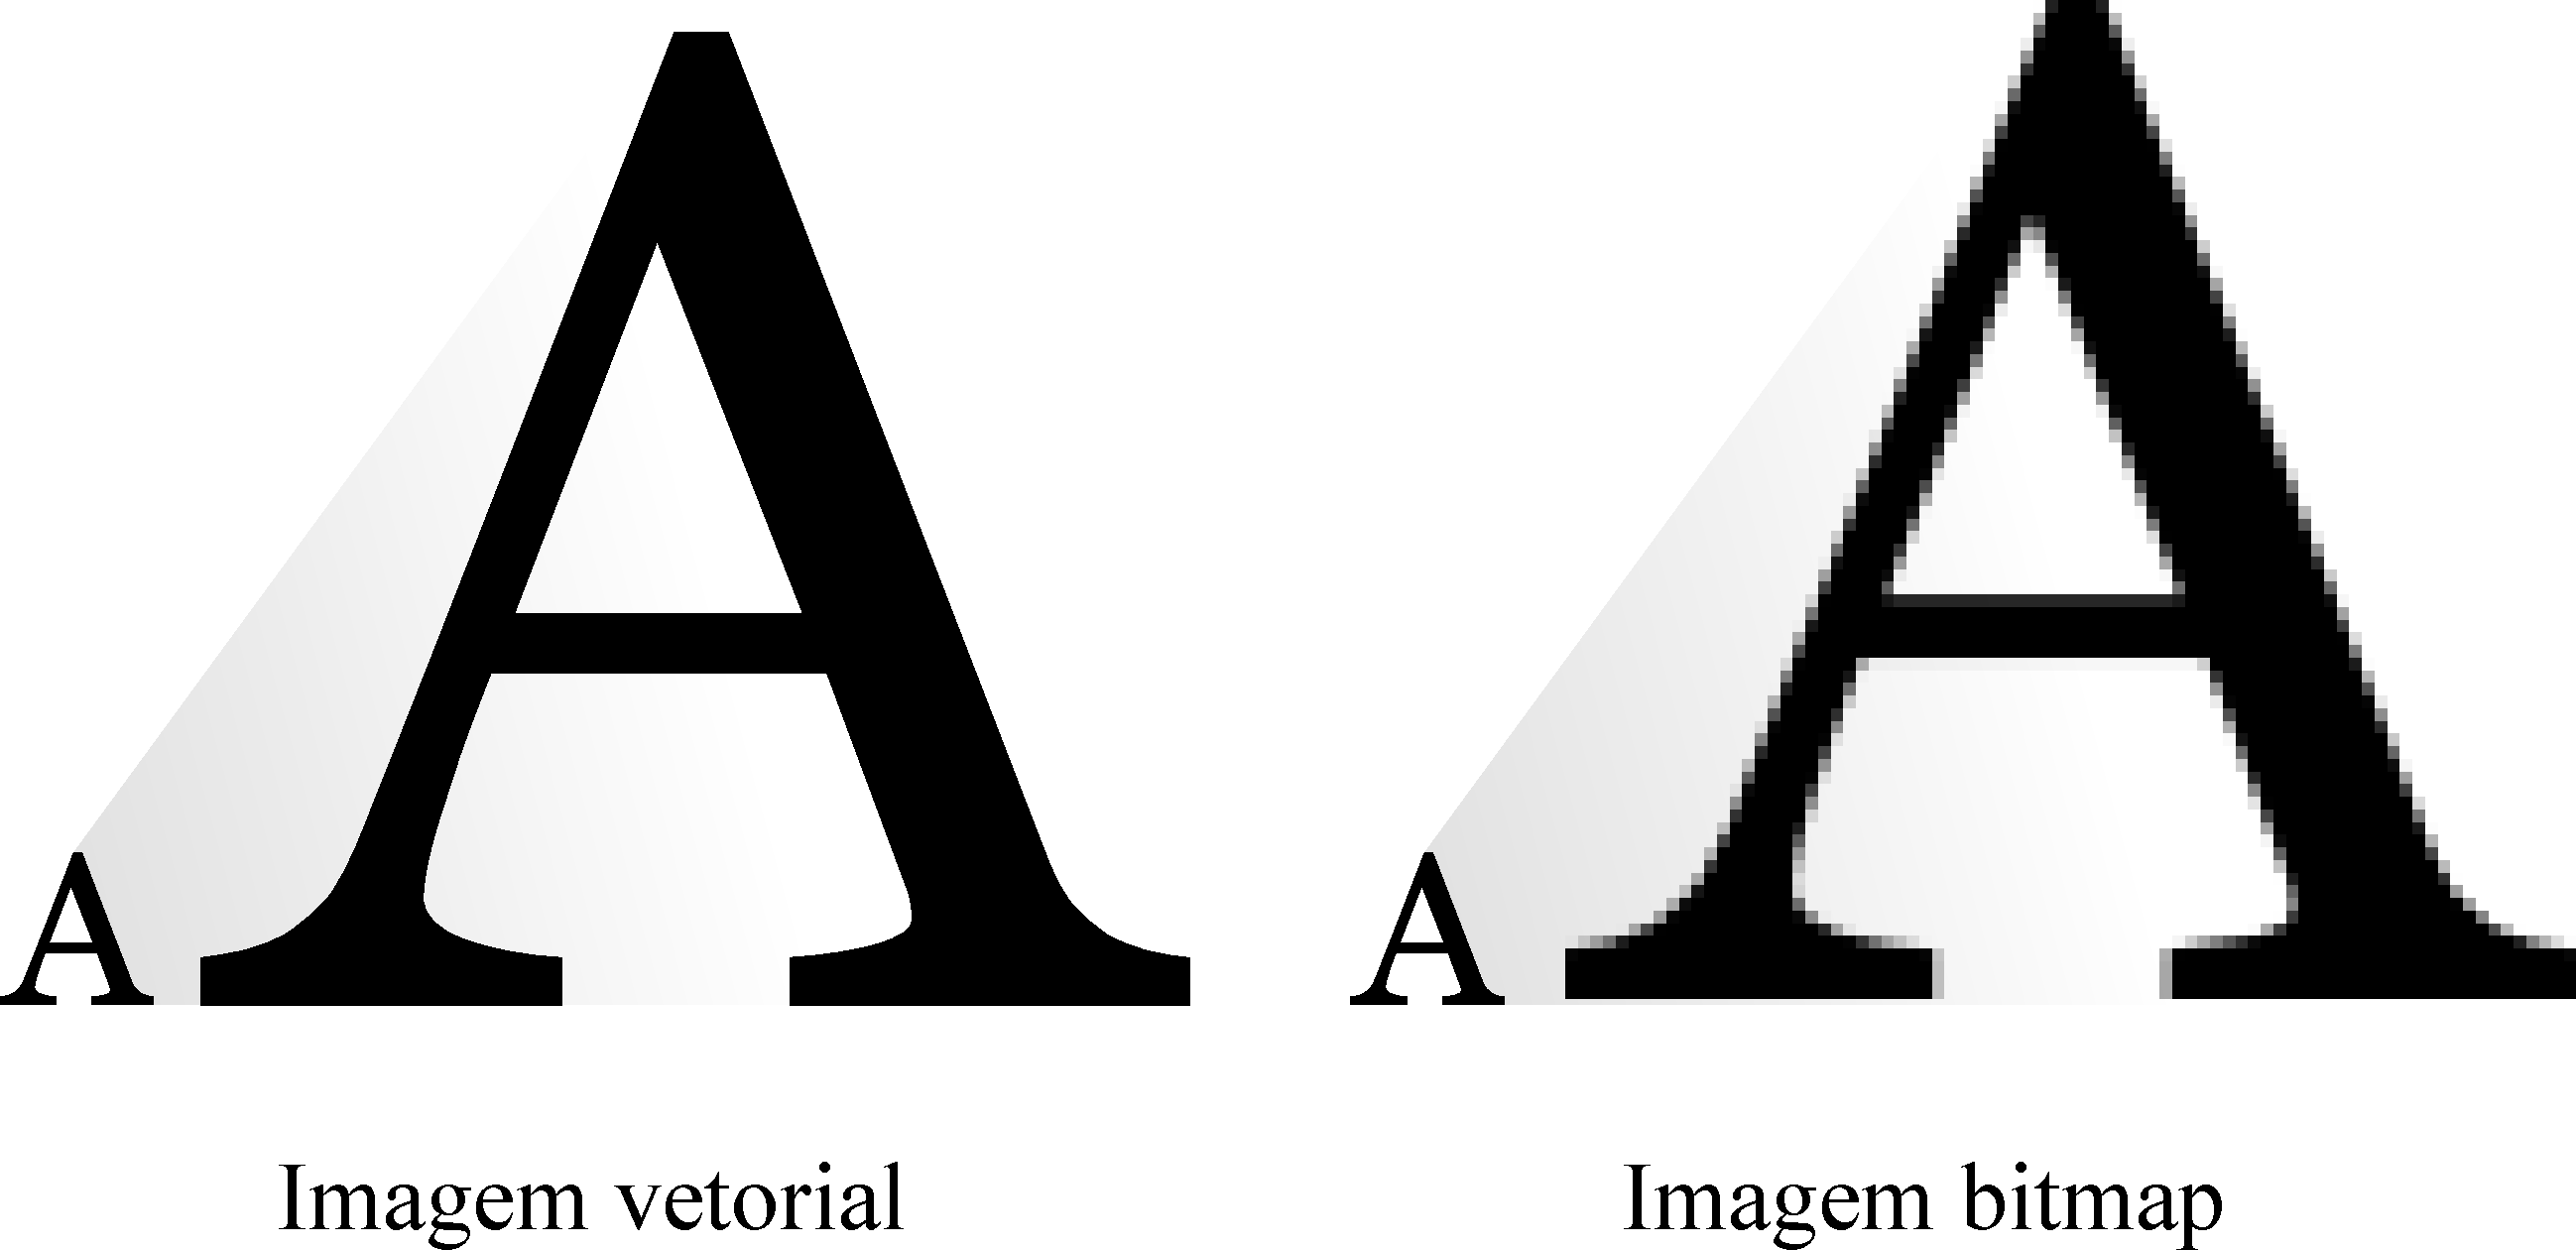
\includegraphics[height=4cm]{imagens/vetor_x_bitmap.pdf}
  \end{center}
  \caption{ Diferença entre uma imagem vetorial e uma imagem \textit{bitmap}.
    Uma imagem \textit{bitmap} perde a qualidade quando ampliada,
    o que não ocorre com uma imagem vetorial }
  \label{fig:vetor_x_bitmap}
\end{figure}

Quanto a cores, existem diversas padrões de representação, a
codificação RGB (sigla para \textit{Red},
\textit{Green}, \textit{Blue}) é a mais comum e define três bytes para armazenar,
respectivamente, o vermelho, o verde e o azul, cada uma sendo um inteiro na
faixa de 0 a 255. Outros padrões de representação são HLS
(sigla para \textit{Hue}, \textit{Lightness}, \textit{Saturation}),
HSB (sigla para \textit{Hue}, \textit{Saturation}, \textit{Brightness}),
HSV (sigla para \textit{Hue}, \textit{Saturation}, \textit{Value}), Hunter Lab,
CIE 1976 Lab e CMYK (sigla para \textit{Cian}, \textit{Magenta},
\textit{Yelow}, \textit{Black}), este último utilizado em mídias impressas.

Embora uma imagem \textit{bitmap} seja armazenada na RAM com todos os \textit{pixels} é comum,
por uma questão de economia de espaço e tempo de trasmissão, a compressão destes
arquivos. Entre todos os formatos de compressão os mais conhecidos são o GIF
(\textit{Graphics Inter-change Format}), o JPEG
(\textit{Joint Photographic Experts Group}) e
o PNG (\textit{Portable Network Graphics}).

Neste trabalho as imagens sempre serão \textit{bitmap}, com as cores codificadas
no padrão RGB e comprimidas no formato JPEG. As imagens serão tratadas como
equações, notacionadas na forma $ f(x,y) $, onde $ x $ e $ y $ são inteiros e indicam a
posição de um \textit{pixel} específico, e os pixels são interpretados como tuplas na
forma $ (r, g, b) $, onde $ r $, $ g $ e $ b $ pertencem ao subintervalo inteiro
de 0 a 255 e representam as cores vermelha, verde e azul respectivamente.

\section{Simplificação de imagens e extração de características}\label{sec:simplificacao_img}

Qualquer método de agrupamento depende sensivelmente do critério de semelhança
adotado nas comparações entre os elementos, será esse critério que, basicamente,
determinará a classe de cada elemento. O critério de semelhança deve ser baseado
em alguma característica mensurável e comparáveis entre sí, ou seja, deve haver
uma forma de se estabelecer a distância entre diferentes valores desta característica.
Esta distância determinará a semelhança entre os elementos, onde
quanto mais próximos mais semelhantes.

Em imagens existem diversas características que servem como critérios de
semelhança, do ponto de vista da percepção humana, estas características são
comumente ligados as cores, texturas ou formas presentes na imagen, ou ainda,
a uma combinação delas. Em relação as cores, medidas de histograma são as mais
populares; em texturas é comum a utilização de momentos do histograma de brilho,
matriz de co-ocorrência, granulometria e informações do aspectro de Fourier;
para formas se destacam os algorítimos de detecção de formas de interesse e os
momentos invariantes; uma abordagem mista de cores e formas é possível atravéz
de modelos de misturas gaussianas.

\section{Momentos invariantes como descritores de imagens}\label{sec:momentos_desc}

Supondo que uma forma particular estaja presente numa imagem $ A $, e que outra
bastante parecida esteja presente numa imagem $ B $, e que em relação a $ A $ a forma
em $ B $ está invertida, ou, para o exemplo ficar mais claro, que esta forma seja a
silhueta de um rosto, que em $ A $ está virado a esquerda e em $ B $ virado a direita,
como indicado na Figura \ref{fig:rostos}, é um objetivo particular deste trabalho que ambas
as imagens possuam descritores (características extraídas) bastante semelhantes,
senão identicos; afinal, em termos perceptivos, ou seja, em termos de significado
que um observador atribui as imagens, neste exemplo $ A $ e $ B $, ambas possuem a
figura de um rosto e estar cada um virado numa direção é uma caracterrística
marginal e não deve influenciar no agrupamento.

\begin{figure}[H]
  \begin{center}
    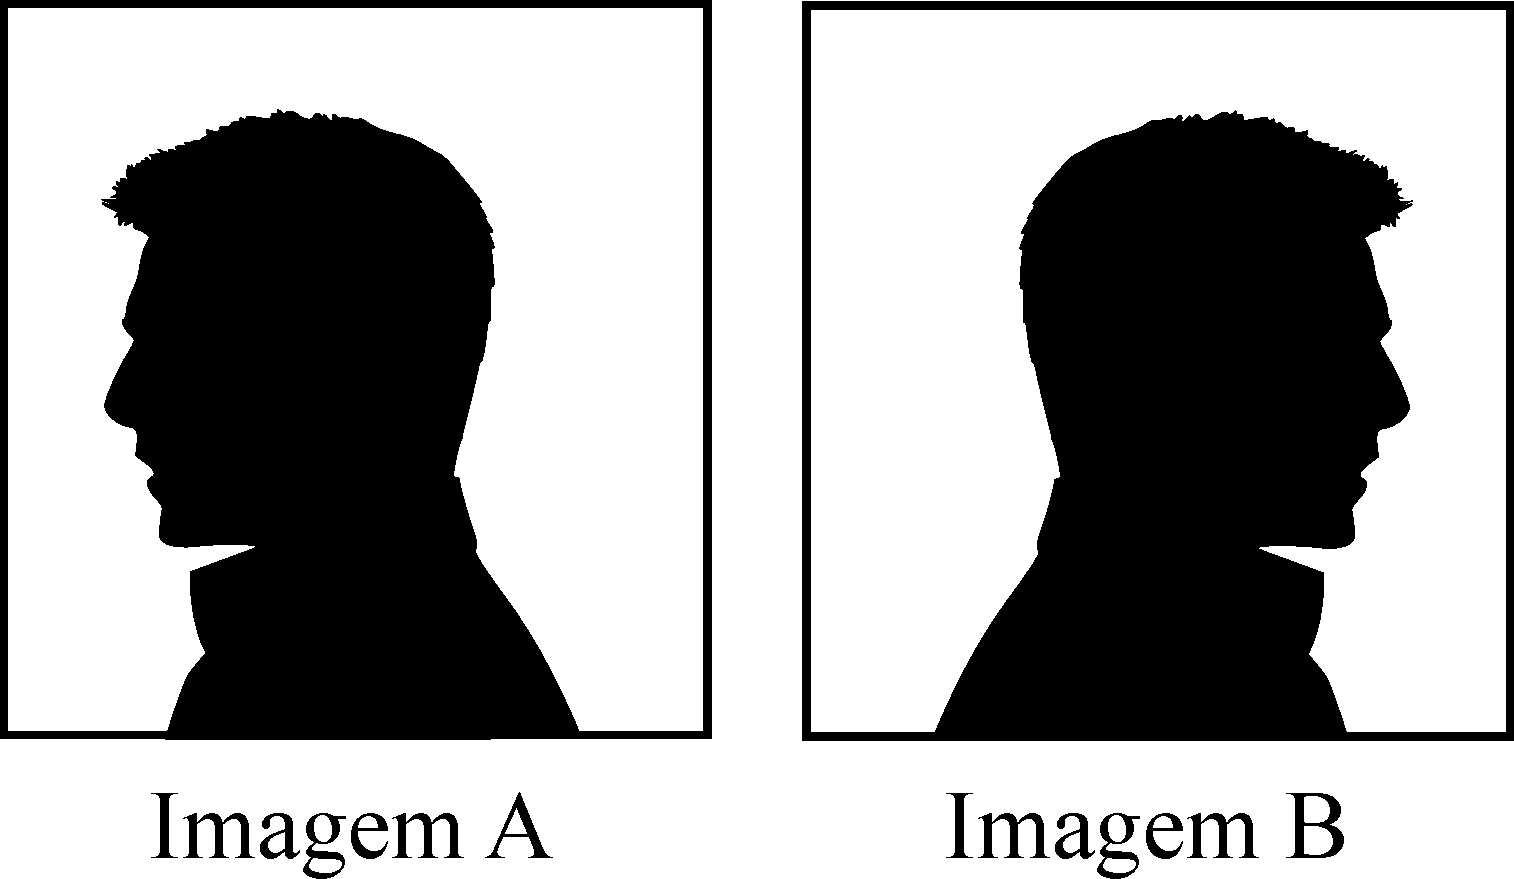
\includegraphics[height=4cm]{imagens/rostos.pdf}
  \end{center}
  \caption{ Duas imagens idênticas porém espelhadas.  }
  \label{fig:rostos}
\end{figure}

O mesmo pode ser dito para rotação, traslação e escala de formas em diferentes
imagens, o que se deseja é a forma em sí, algo como seu protótipo, independente
destas trasformações, como indica a Figura \ref{fig:carros_transformados}.
A pretenção é, ao se descartar estas transformações,
simular o que aparentemente é o comportamento natural de um indivíduo ao, sem
ajuda do computador, categorizar e agrupar imagens.

\begin{figure}[H]
  \begin{center}
    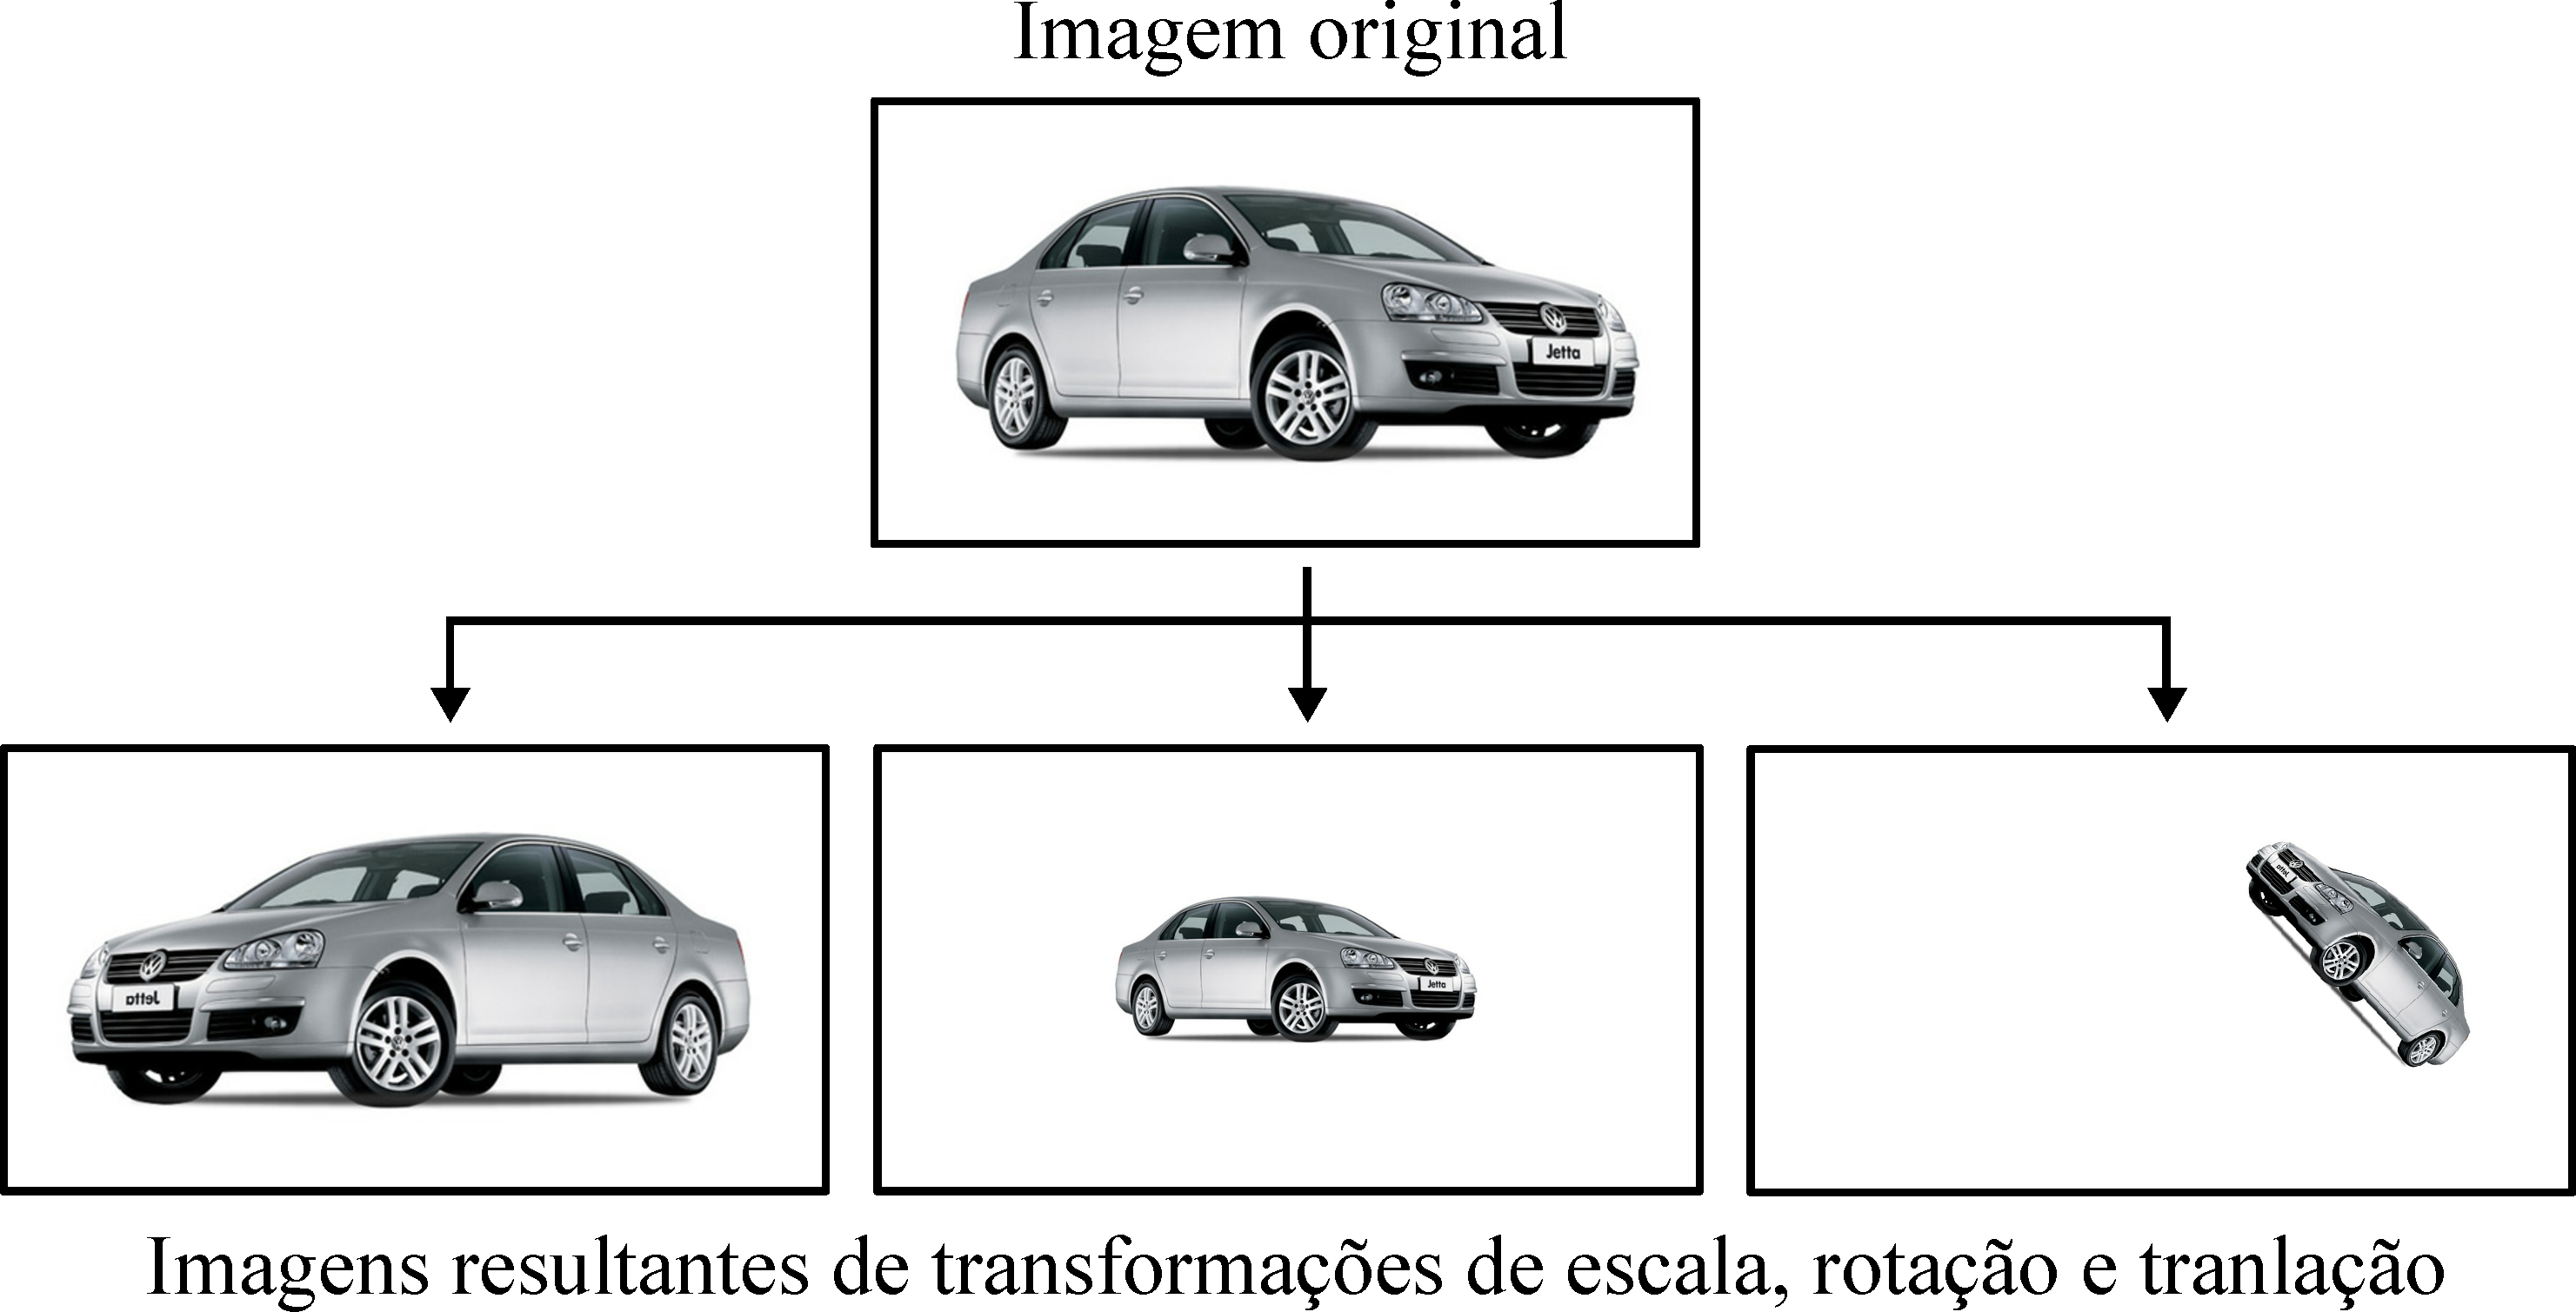
\includegraphics[height=7cm]{imagens/carros_transformados.pdf}
  \end{center}
  \caption{ Exemplos de transformações de rotação, translação e escala sobre
    uma imagem, e como elas não alteram a essência das formas presentes na
    imagem original. }
  \label{fig:carros_transformados}
\end{figure}

Um conjunto de descritores atende aos propósitos indicados acima, são os
descritores de Hu, mais comumente chamados de momentos invariantes. Os momentos
invariantes são um conjunto de sete descritores reais que independem de rotação,
translação ou escala, isto é, quando aplicados a uma forma qualquer retornará
os mesmos valores se aplicado a outra forma resultande de uma das três
transformações citadas, ou até mesmo de uma combinação delas.

\subsection{Formulação matemáticas dos momentos invariantes}\label{sec:momentos_mat}

Passemos então agora para formalização matemática desses momentos.

O momento bidimensional de ordem $ (p+q) $ é dado pela
equação \ref{eq:mm_bid_cont}:

\begin{equation}\label{eq:mm_bid_cont}
m_{pq} = \iint x^p y^q f(x, y) \mathrm{d}x \mathrm{d}y, p, q \in
\end{equation}

A equação num domínio discreto, pode ser reescrita na forma:

\begin{equation}\label{eq:mm_bid_disc}
m_{pq} = \sum_{x, y} x^p y^q f(x, y), p, q \in
\end{equation}

A massa total da função $ f(x, y) $ é determinado pelo
momento $ m_{00} $, conforme a equação \ref{eq:mm_bid_m00}:

\begin{equation}\label{eq:mm_bid_m00}
m_{pq} = \sum_{x, y} f(x, y), p, q \in
\end{equation}

Existe um ponto no qual a aplicação pontual da massa total gera o mesmo momento
que a massa distribuída, este ponto é dito centroide de $ f(x, y) $ e suas
coordenadas $ x $ e $ y $ são dadas pela equação \ref{eq:ct_xy}:

\begin{subequations}\label{eq:ct_xy}
\begin{align}
    \bar{x} = \frac{1}{ m_{00} } \sum x f(x, y) = \frac{ m_{10} }{ m_{00} } \\
    \bar{y} = \frac{1}{ m_{00} } \sum y f(x, y) = \frac{ m_{01} }{ m_{00} }
\end{align}
\end{subequations}

O momento central é obtido se deslocando a imagem para o centroide,
da seguinte forma:

\begin{equation}\label{eq:mm_ctr}
\mu_{pq} = \sum_{x, y} (x - \bar{x})^p (y - \bar{y})^q f(x, y)
\end{equation}

Ainda é necessário normalizar o momento para que os valores resultantes não sejam
extremos a ponto de serem ignorados pelo sistema de reconhecimento de padrões. O
momento central de ordem $ (p+q) $ normalizado é obtido dividindo o momento
central de $ y $ mesma ordem por um fator definido por $ \mu_{00}^\gamma $ ,
conforme indicado pela equação \ref{eq:mm_norm}:

\begin{subequations}\label{eq:mm_norm}
\begin{align}
    \gamma = 1 + \frac{ p + q }{2} \\
    \eta_{pq} = \frac{ \mu_{pq} }{ \mu_{00}^\gamma }
\end{align}
\end{subequations}

A partir dessas equações são estabelecidos sete momentos invariantes à translação,
 rotação e escala, chamados de momentos de Hu, ou descritores de Hu. São eles:

\begin{subequations}\label{eq:mmt}
\begin{align}
  \varphi_1 = \eta_{20} + \eta_{02} \\
  \varphi_2 = (\eta_{20} - \eta_{02})^2 + 4\eta_{11}^2\\
  \varphi_3 = (\eta_{30} - 3\eta_{12})^2 + (3\eta_{21} - \eta_{03})^2\\
  \varphi_4 = (\eta_{30} + \eta_{12})^2 + (3\eta_{21} + \eta_{03})^2 \\
%
  \begin{tabular}{r c l}
    \(\varphi_5\) & \(=\) & \((\eta_{30} - 3\eta_{12})(\eta_{30} + \eta_{12}) \left[ (\eta_{30} + \eta_{12})^2 - 3(\eta_{21} + \eta_{03})^2 \right]\) \\
                  & \(+\) & \((3\eta_{21} - \eta_{03})(\eta_{21} + \eta_{03}) \left[ 3(\eta_{30} + \eta_{12})^2 - (\eta_{21} + \eta_{03})^2 \right]\)
  \end{tabular}\\
%
  \begin{tabular}{r c l}
    \(\varphi_6\) & \(=\) & \((\eta_{20} - \eta_{02})\left[ (\eta_{30} + \eta_{12})^2 - (\eta_{21} + \eta_{03})^2 \right]\)\\
                  & \(+\) & \(4\eta_{11}(\eta_{30} - \eta_{12})(\eta_{21} + \eta_{03})\)
  \end{tabular}\\
%
  \begin{tabular}{r c l}
    \(\varphi_7\) & \(=\) & \((3\eta_{21} - \eta_{30})(\eta_{30} + \eta_{12})\left[ (\eta_{30} + \eta_{12})^2 - 3(\eta_{21} + \eta_{03})^2 \right]\)\\
                  & \(+\) & \((3\eta_{12} - \eta_{03})(\eta_{21} + \eta_{03})\left[ 3(\eta_{30} + \eta_{12})^2 - (\eta_{21} + \eta_{03})^2 \right]\)
  \end{tabular}
\end{align}
\end{subequations}

Observe que os momentos são definidos para um ponto de valor discreto, isto implica que
devemos abandonar qualquer descriçao vetorial de cores, neste caso, devemos
passar uma cor do formato RGB para seu tom de cinza. Neste trabalho o tom de
cinza para uma cor RGB é o valor médio para os canais vermelhor, verde e azul.

\section{Binarização de imagens}\label{sec:binarizacao_img}

Mesmo que os momentos invariantes sejam, a princípio, bons descritores, eles
não podem ser extraídos sem que a imagem tenha passado por algumas
transformações. Estas transformações não são obrigatórias, isto é, não são
restrições necessárias a aplicação dos momentos, mas são transformações que
fazem sentido no processo de agrupamento, mais especificamente, no subprocesso
de extração de características relevantes.

É perfeitamente válido supor que nem todas os \textit{pixels} de uma imagem sejam
relevantes, ou no mínimo, que determinados \textit{pixels} são mais relevantes
que outros, estes \textit{pixels} mais relevantes podem ser interpretados
como regiões de interesse, isto é, regiões que despertam maior atenção dos
observadores. Em suma, podemos dividir a imagem em duas regiões, uma de
interesse chamada de primeiro plano (\textit{foreground}) e outra que pode ser
negligenciada chamada plano de fundo (\textit{background}), como no exemplo
da Figura \ref{fig:girafa_limiarizacao}. A separação entre
essas duas regiões é chamado de limiarização, ou ainda, remoção de fundo.

\begin{figure}[H]
  \begin{center}
    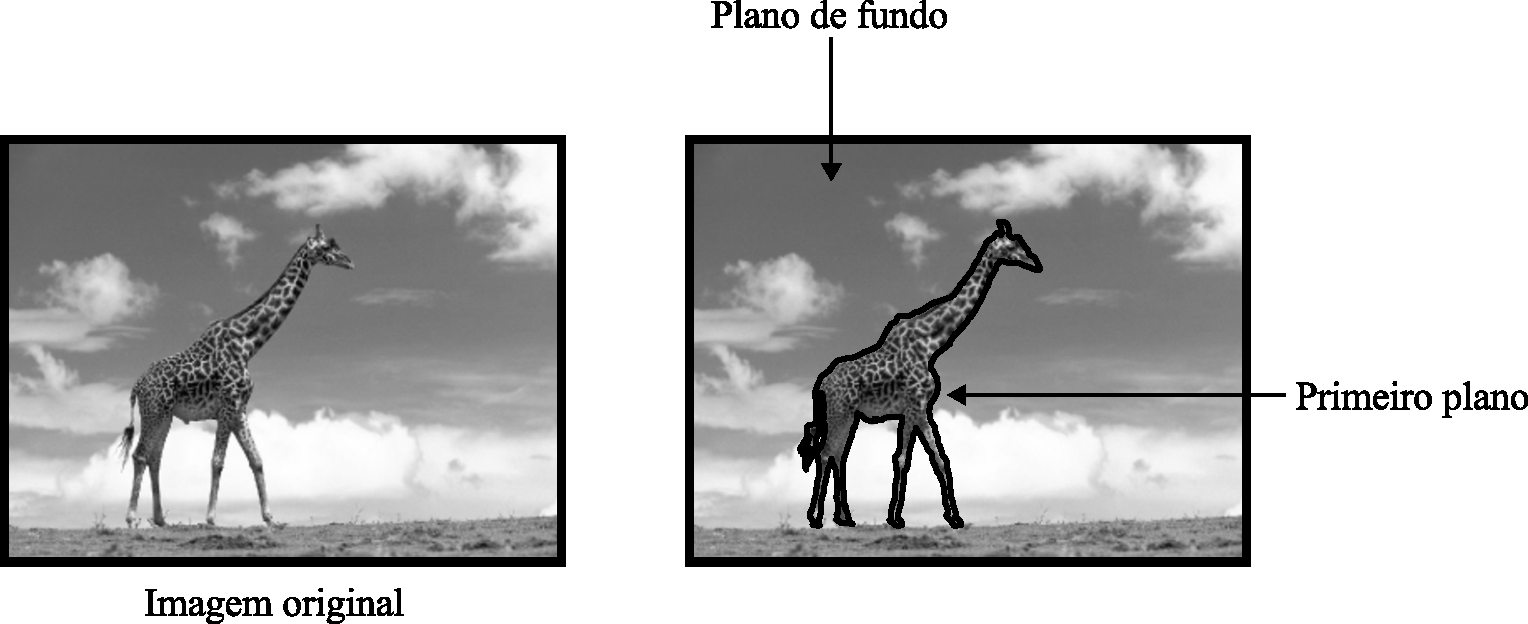
\includegraphics[height=6cm]{imagens/girafa_limiarizacao.pdf}
  \end{center}
  \caption{ Imagem com o primeiro plano e o plano de fundo destacados. }
  \label{fig:girafa_limiarizacao}
\end{figure}

Extrair da imagem os momentos invariantes apenas do primeiro plano
torna os descritores mais interessantes para classificação, afinal, os valores
ficam restritos apenas a região de maior interesse, sendo o plano de fundo
totalmente ignorado na extração destas características.

Outro ponto a ser considerado, como visto na seção anterior, é que
a extração dos momentos depende da intensidade de
cada \textit{pixel}, de modo que uma variação na intensidade de um \textit{pixel}
interfere no resultado dos momentos. Como agora apenas o primeiro plano é
aplicado na extração, apenas as variações de intensidade nesta região são
consideradas; contudo, estas variações podem em determinadas ocasiões gerar
momentos muito distintos para regiões que, morfologicamente, são bem parecidas.
Suponha o caso de, por exemplo, duas imagens que no primeiro plano apresentam a
figura de uma flor, como na Figura \ref{fig:flor_mmt}, na primeira a flor
tem a coloração clara, e na segunda escura, ao aplicar o momento sobre estas
duas imagens, mesmo que tenham uma forma bem parecida, teremos resultados
significativamente diferentes para os momentos das duas. É desejável eliminar
este tipo de discrepância, isto é possível tornando todas as informações da
primeiro plano homogêneas, ou seja, fazer com que cada \textit{pixel} do
primeiro plano tenha o mesmo peso para extração dos momentos. Esta homogenização
sobre uma imagem já limiarizada é chamada de
binarização, isto porque teremos duas regiões, uma irrelevante onde
cada \textit{pixel} terá o valor nulo, e outra relevante onde cada \textit{pixel}
terá seu máximo valor.

\begin{figure}[H]
  \centering

  \begin{subfigure}{0.3\textwidth}
    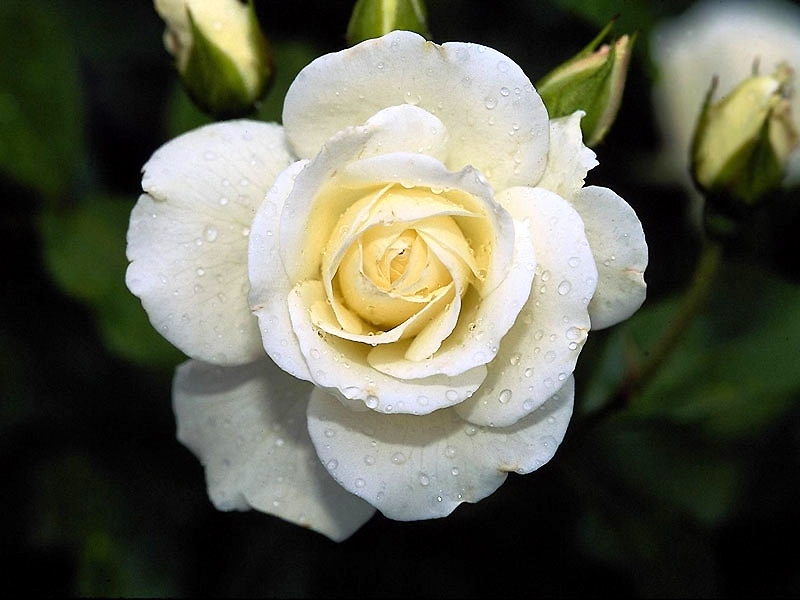
\includegraphics[width=\textwidth]{imagens/flor_branca.jpg}
    \caption{Rosa branca}
    \label{fig:flor1}
  \end{subfigure}~
  \begin{subfigure}{0.3\textwidth}
    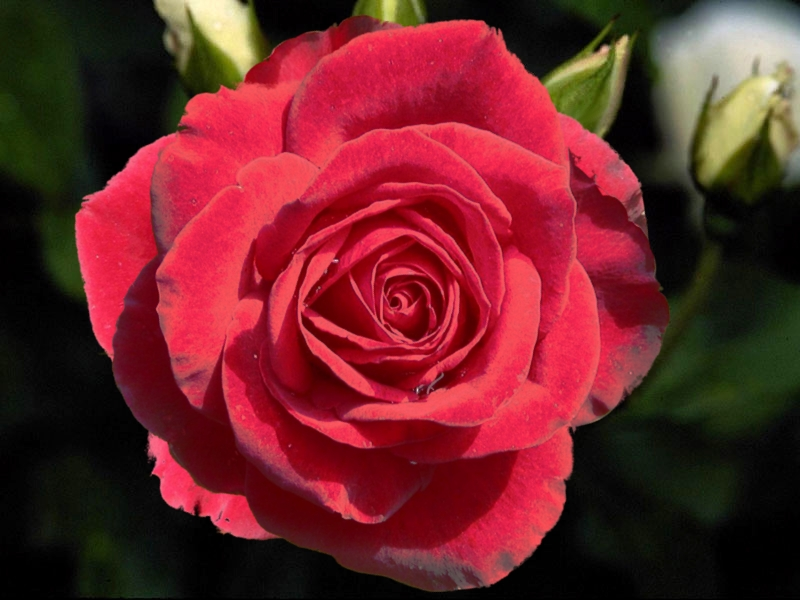
\includegraphics[width=\textwidth]{imagens/flor_vermelha.jpg}
    \caption{Rosa vermelha}
    \label{fig:flor2}
  \end{subfigure}~

  \begin{subfigure}{0.3\textwidth}
    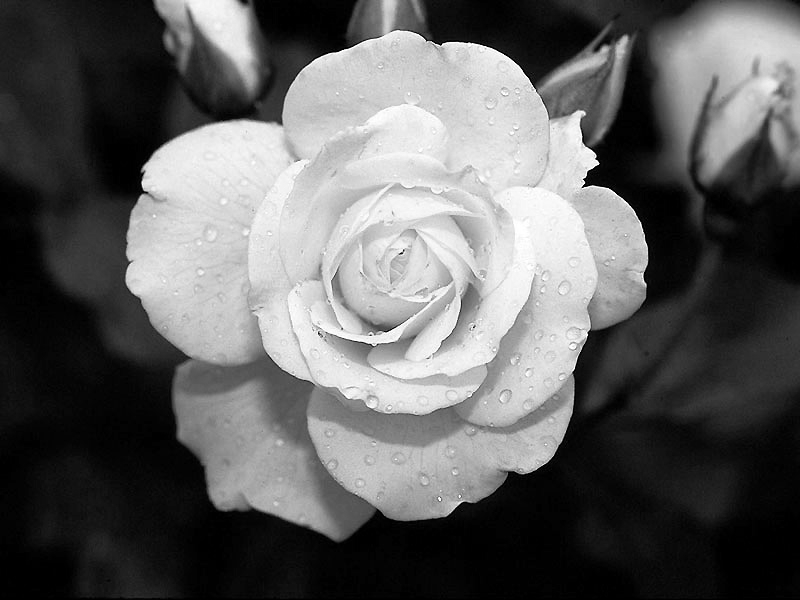
\includegraphics[width=\textwidth]{imagens/flor_branca_pb.jpg}
    \caption{Rosa branca em tons de cinza}
    \label{fig:flor3}
  \end{subfigure}~
  \begin{subfigure}{0.3\textwidth}
    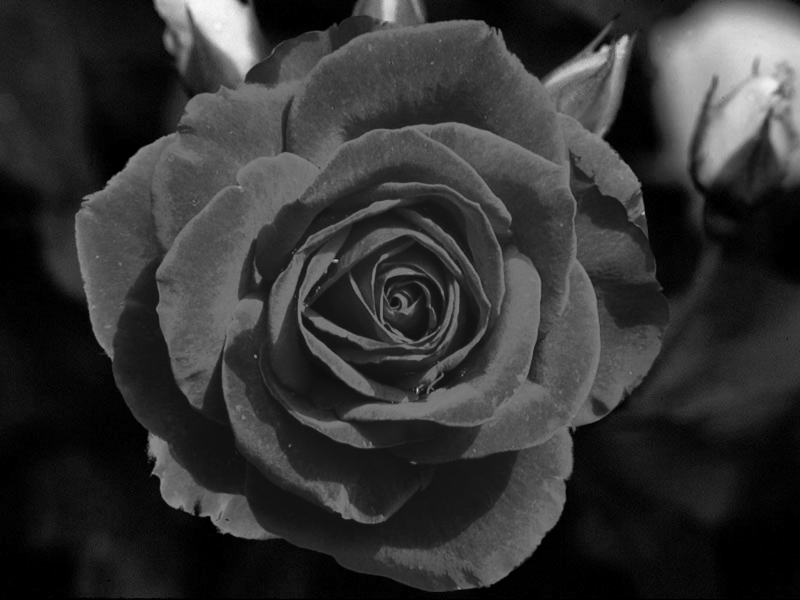
\includegraphics[width=\textwidth]{imagens/flor_vermelha_pb.jpg}
    \caption{Rosa vermelha em tons de cinza}
    \label{fig:flor4}
  \end{subfigure}

  \caption{ Imagens visualmente semelhantes mas com relativa diferença nos
    valores dos momentos devido as grande diferença de tons no primeiro plano. }
  \label{fig:flor_mmt}
\end{figure}

Binarizar uma imagem, o que implicitamente também implica em limiarizá-la, é
um processo bem simples e pode ser feito apenas como base no histograma. O que
se deseja é anular todos os \textit{pixels} abaixo de um limiar e
potencializar os que estão acima dele. Como indicado no Algoritmo \ref{alg:binarizacao_imagem}:

\begin{algorithm}[H]
\caption{Binarização de uma imagem}\label{alg:binarizacao_imagem}
\SetAlgoRefName{alg:binarizacao_imagem}
\Entrada{$ f(x, y) $ , $ l $ }
\Inicio{
  \ParaCada{$ p \in f(x, y) $}{
    \eSe{$ p < l $}{
      $ p \gets 0 $
    }{
      $ p \gets 255 $
    }
  }
}
\end{algorithm}

Contudo, o Algorítimo \ref{alg:binarizacao_imagem} não indica como definir o limiar
ótimo, isto é, aquele que melhor separa o primeiro plano do plano de fundo, esta
operação é realizada, neste trabalho, através do método de Otsu, descrito na próxima seção.

\section{Método de Otsu}\label{sec:metodo_otsu}

O método de Otsu é um método de \textit{thresholding} global, isto é, o valor obtido é
uma constante, para escolha do melhor limiar. A base deste método é sua interpretação
do histograma como como uma função de densidade de probabilidade
discreta, da seguinte maneira:

\begin{equation}\label{eq:histograma_norm}
  p_r(r_q) = \frac{n_q}{n}, q = 0, 1, 2, ..., L-1
\end{equation}

Onde:

\begin{itemize}
  \item $ n $ é o total de \textit{pixels} da imagem;
  \item $ n_q $ é o total de \textit{piixels} que tem intensidade $ r_q $ e
  \item $ L $ é o total de níveis de intensidade na imagem.
\end{itemize}

O método de Otsu escolhe o limiar de valor $ k $, tal que $ k $ é um nível de
intensidade que divide o histograma em duas classes
$ C_0 = [0, 1, ..., k-1] $ e $ C_1 = [k, k+1, ..., L-1] $, e que maximise a
variância $ \sigma_{B}^2 $ definida como:

\begin{equation}\label{eq:maximizacao_variancia}
  \sigma_{B}^2 = \omega_0(\mu_0 - \mu_T)^2 + \omega_1(\mu_1 - \mu_T)^2
\end{equation}

Sendo:

\begin{subequations}\label{eq:somatorios_maximizacao}
\begin{align}
  \omega_0 = \sum_{q=0}^{k-1} p_q(r_q)\\
  \omega_1 = \sum_{q=k}^{L-1} p_q(r_q)\\
     \mu_0 = \sum_{q=0}^{k-1} \frac{qp_q(r_q)}{\omega_0}\\
     \mu_1 = \sum_{q=k}^{L-1} \frac{qp_q(r_q)}{\omega_1}\\
     \mu_T = \sum_{q=0}^{L-1} qp_q(r_q)
\end{align}
\end{subequations}

O resultado da binarização com limiar ajustado segundo o método de Otsu pode
ser observado na Figura \ref{fig:bin_otsu}

\begin{figure}[H]
  \centering

  \begin{subfigure}{0.3\textwidth}
    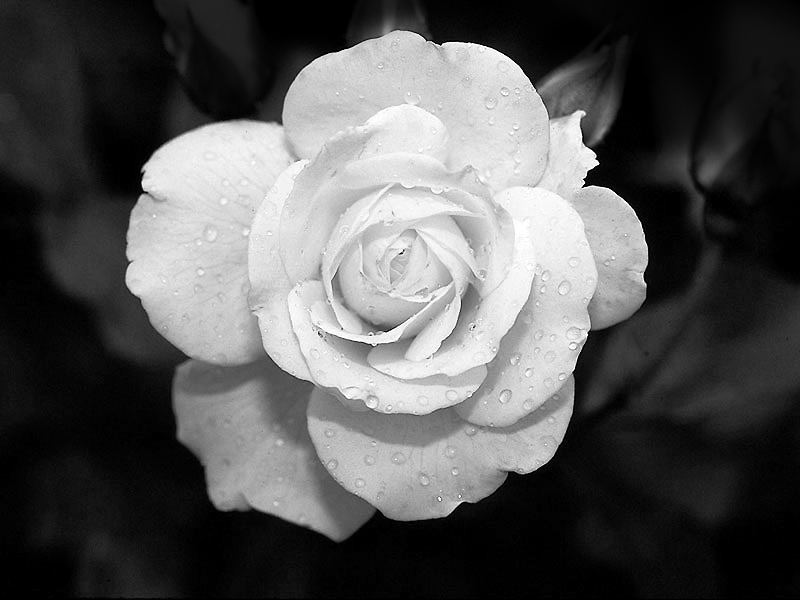
\includegraphics[width=\textwidth]{imagens/flor_branca_pb2.jpg}
    \caption{Imagem original}
    \label{fig:flor1}
  \end{subfigure}~
  \begin{subfigure}{0.3\textwidth}
    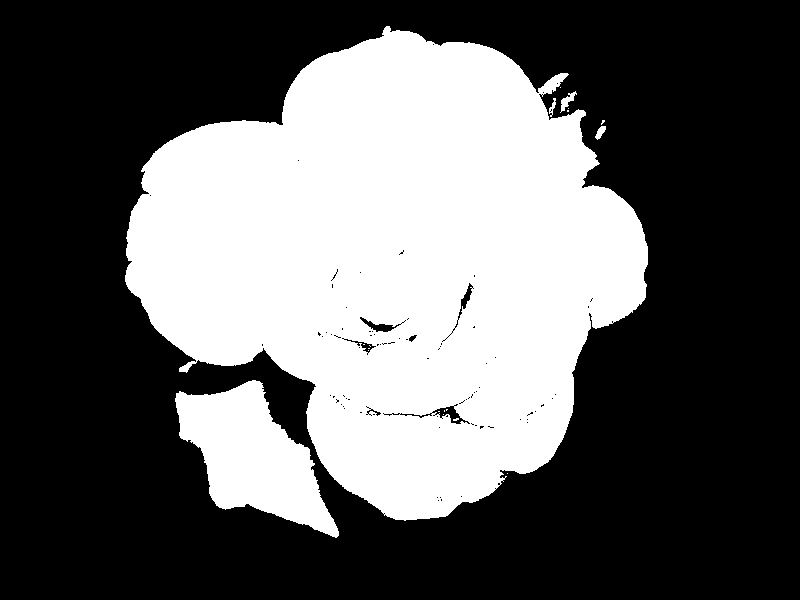
\includegraphics[width=\textwidth]{imagens/flor_branca_pb2_lm.jpg}
    \caption{Imagem binarizada}
    \label{fig:flor2}
  \end{subfigure}~

  \caption{ Imagem binarizada com limiar definito pelo método de Otsu. }
  \label{fig:bin_otsu}
\end{figure}

\section{Resumo do processo de extração de características}
\label{sec:resumo_extracao_caracteristicas}

Como discutido nas seções anteriores deste capítulo, os momentos invariantes
foram eleitos como os descritores a serem utilizadas para determinar a
similaridade entre as imagens, contudo, estes descritores são extraídos somente
após as imagens terem passado por determinadas transformações que visam
simplificá-las e potencializar as regiões de maior interesse, e assim, produzir
valores mais significativos para os momentos. As transformações  aplicadas as
imagens são a dessaturação e a binarização, nesta ordem.

Podemos resumir visualmente o processo de extração de característica na
Figura \ref{fig:extracao_caracteristicas}:

\begin{figure}[H]
  \begin{center}
    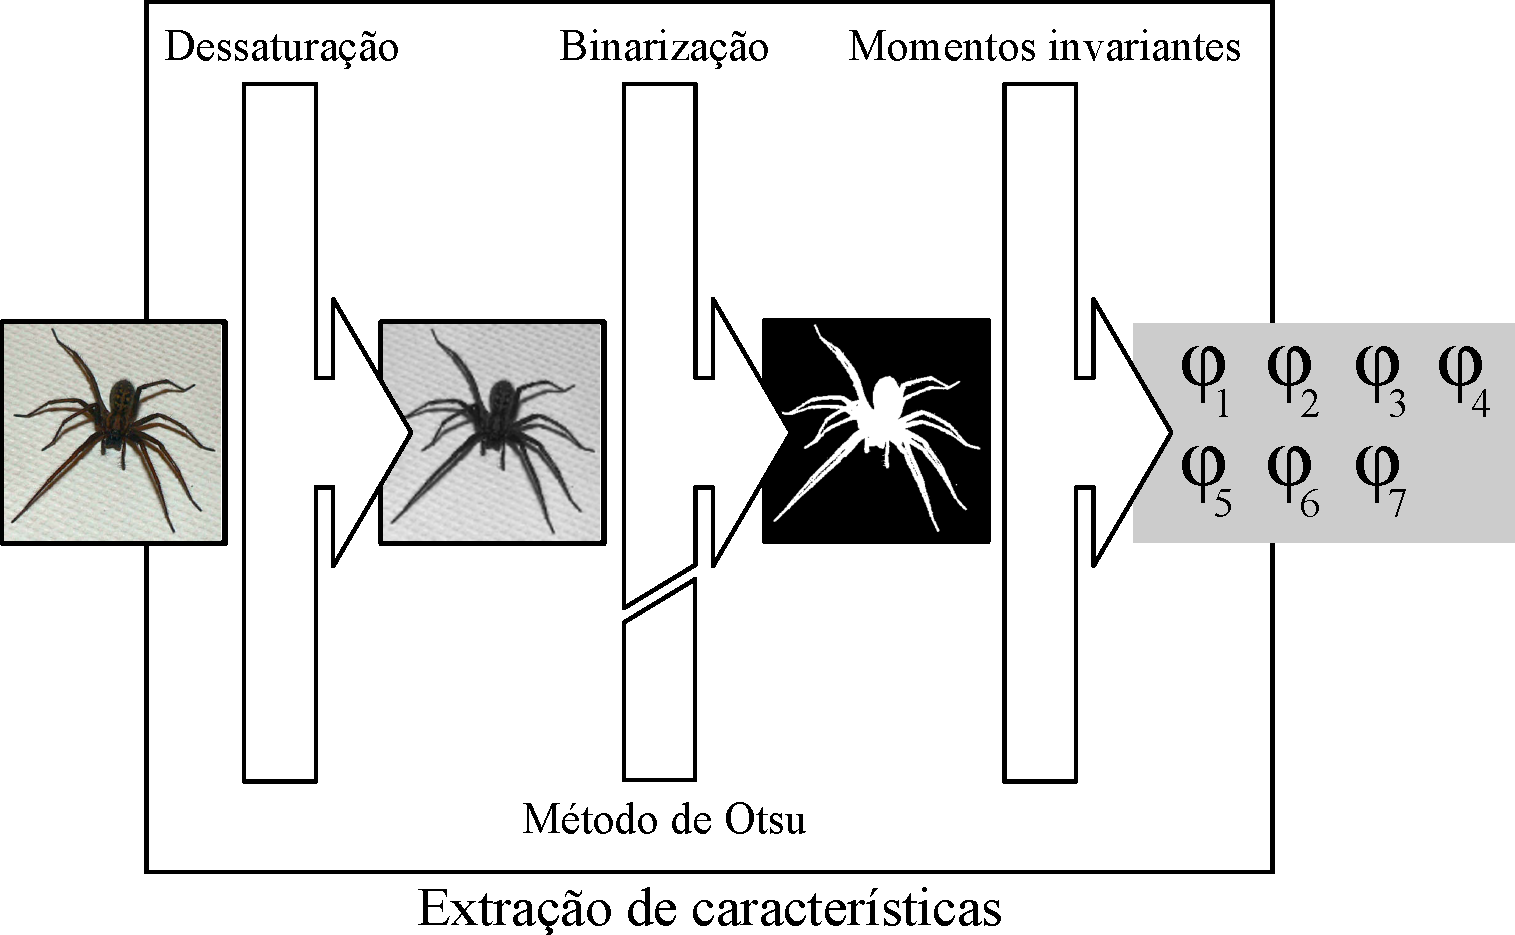
\includegraphics[height=8cm]{imagens/extracao_caracteristicas.pdf}
  \end{center}
  \caption{ Esquema do processo de extração de caracteristicas. }
  \label{fig:extracao_caracteristicas}
\end{figure}

\chapter{Rotulação das imagens}

No capítulo anterior foi apresentado o conjunto de características que serão
utilizadas para descrever as imagens, e como este conjunto de características é
extraído. Neste capítulo o objetivo é demostrar como este conjunto de
características é processado de modo a classificar e agrupar as imagens. As
redes neurais de Kohonen são o conceito chave deste processo, contudo, como
será visto, um conjunto de técnicas auxiliares também são necessárias para
estruturar o \textit{clustering}.

\section{Mapas auto organizáveis}\label{sec:mapas_aut_organizaveis}

A maneira mais intuitiva de se agrupar imagens, ou qualquer outro tipo de
informação, é estabelecer um determinado número de classes e mapear cada imagem
para uma das classes, de modo que imagens semelhantes pertençam a mesma classe.
Entretanto, este tipo de abordagem desconsidera graus diferentes de semelhança
intra-classes, e até mesmo, graus diferentes de semelhança inter-classes, isto
é, havendo somente a ligação das imagens com suas classes como será possível
determinar, numericamente, o quão semelhante duas imagens são? Ou até mesmo,
quão diferentes são duas classes uma da outra?

Estas perguntas são relevantes porque, para os casos onde uma classe possui
centenas de imagens, muitas vezes o que se deseja é apenas uma amostra
significativa da classe, ou em outra situação, estando em pesse de uma
determinada imagem, deseja-se um número definido de imagens similares. Por isto,
um método voltado exclusivamente para agrupamentos pode não fornecer um conjunto
adequado de parâmetros que permitam extrair das classes informações como as
necessárias para responder as questões acima.

Partindo de um outro ponto, em vez de iniciar o projeto do \textit{clusterig} pelas
classes, mas sim pela distância entre as imagens, surge a possibilidade de criar
espaços para posicionar as imagens e, tendo a distância como medida de
diferença, definir as classes como regiões ou intervalos dentro destes espaços.
Deste modo, as classes não serão um parâmetro para a classificação, elas serão
definidas automaticamente pela dispersão das imagens nestes espaços através de
um processo dinâmico e automático. O resultado será não somente um método que
agrupa imagens mas que também define, sem a participação ativa do usuário, as
próprias classes utilizadas no agrupamento.

Estes espaços onde as imagens serão posicionadas podem ser de qualquer dimensão,
contudo, um espaço bidimensional de intervalos discreto é o suficiente para os
propósitos deste trabalho. Outro ponto importante é que estes espaços não podem
ser infinitos, pois obviamente estão limitados pela memória e pela capacidade
de processamento do computador, por isto, serão utilizados sempre espaços
limitados. Em resumo, podemos chamar estes subespaços bidimensionais discretos
de mapas, onde cada ponto é uma posição potencial para uma imagem, e as imagens
estão tão próximas quanto forem semelhantes.

Em resumo, a localização espacial de cada imagem e sua vizinhança topológica
representam, em um domínio ou característica particular, nestes casos os
momentos invariantes, uma classe, e estas classes são construídas de forma
emergente, sem nenhuma comparação com padrões desejados, por isto são ditos
auto organizáveis, como indica a Figura \ref{fig:mapa_classes_dist}.

\begin{figure}[H]
  \begin{center}
    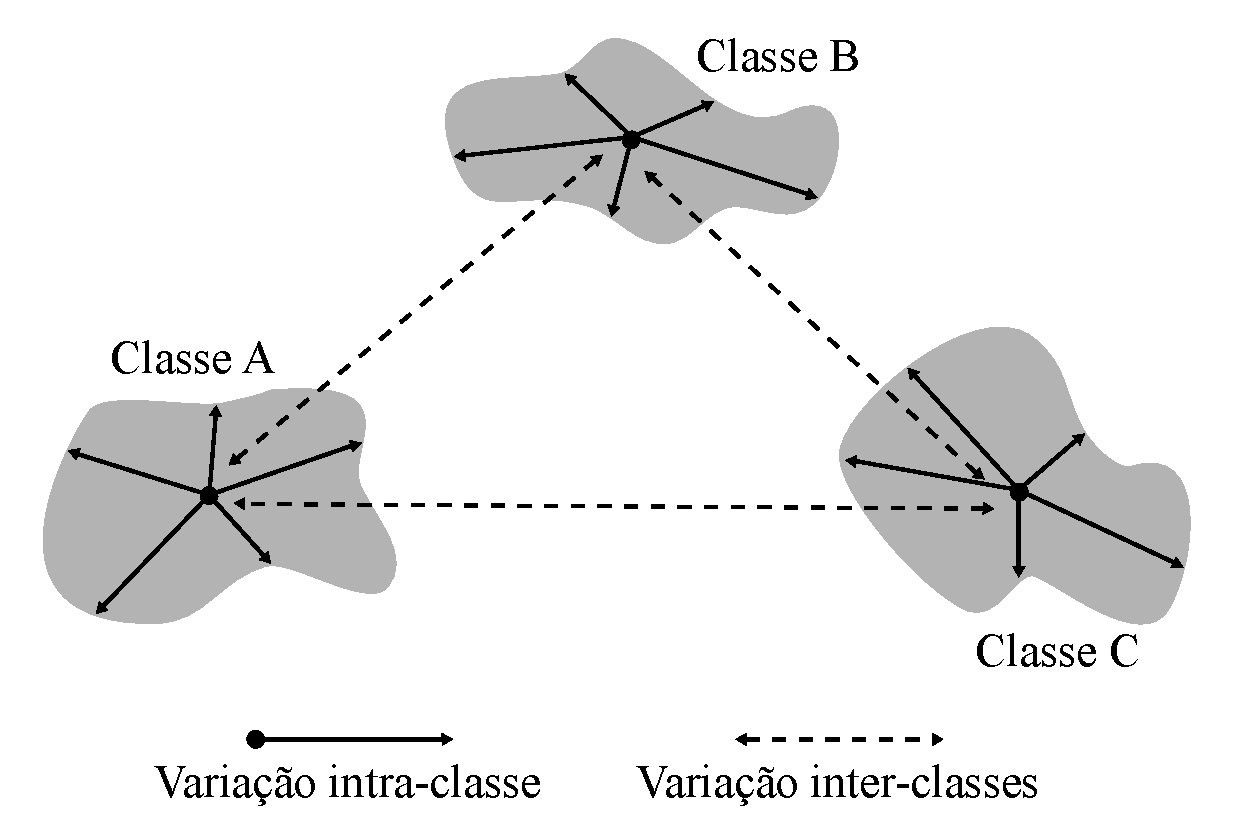
\includegraphics[height=6cm]{imagens/mapa_classes_dist.pdf}
  \end{center}
  \caption{ Organização das classes em um mapa auto organizável, coesão interna
    entre os elementos e isolamento externo entre as classes. }
  \label{fig:mapa_classes_dist}
\end{figure}

\section{Redes de Kohonen como mapa auto organizável}\label{sec:redes_kohonen_mapas}

Dentro da Inteligência artificial, mais especificamente no contexto do
aprendizado de máquina, as redes neurais artificiais são sistemas computacionais
inspirados na estrutura do cérebro, em particular dos neurônios, que adquirem
conhecimento através da experiência.

As redes neurais se assemelham a grafos direcionados, onde os nós são os
neurônios, ou unidades de processamento, que possuem uma quantidade indefinida
de conexões de entrada e saída. As conexões são o equivalente às arestas do
grafo, e são responsáveis por transmitir informações entre os neurônios, podendo
amplificar ou reduzir a acuidade destas informações. A Figura \ref{fig:neuronio}
apresenta o esquema típico de um neurônio.

\begin{figure}[H]
  \begin{center}
    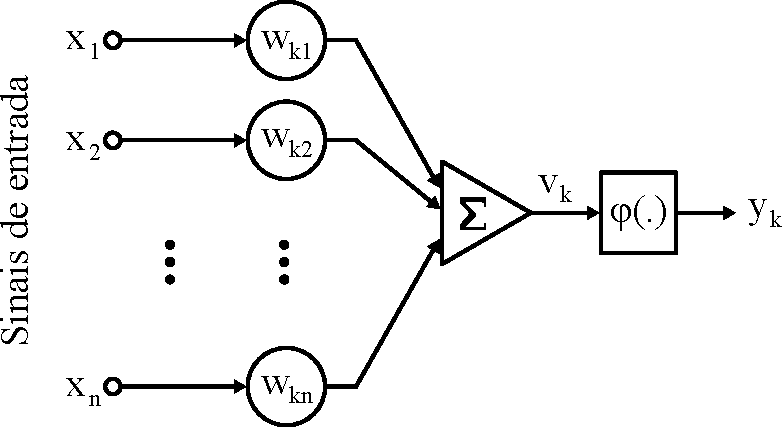
\includegraphics[height=4cm]{imagens/neuronio.pdf}
  \end{center}
  \caption{ Modelo de neurônio. }
  \label{fig:neuronio}
\end{figure}

Sinais de entrada provenientes de fora da rede chegam por meio de conexões
originadas do mundo externo, de modo semelhante, saídas da rede para o mundo
externo são conexões que deixam a rede.

A configuração da rede, ou seja, os peso atual das conexões, determina como os
dados de entrada irão ativar os diferentes neurônios e gerar um determinado
resultado. Para grande maioria dos tipos de redes neurais, uma configuração
particular é obtida através de um algoritmo de treinamento. O treinamento em
geral busca reforçar as conexões que geram bons resultados e penalizar as que
não geram.

As redes de Kohonen apresentam apenas duas camadas de neurônios, a camada de
entrada e a de saída. A camada de saída é uma espécie de malha de neurônios não
conectados entre si, mas amplamente conectados com os neurônios da camada de
entrada, como indicado na Figura \ref{fig:kohonen}. Esta malha funciona como um
mapa, onde para cada padrão de entrada
apenas um neurônio é ativado, padrões semelhantes ativam neurônios dentro de
uma mesma região da malha.

\begin{figure}[H]
  \begin{center}
    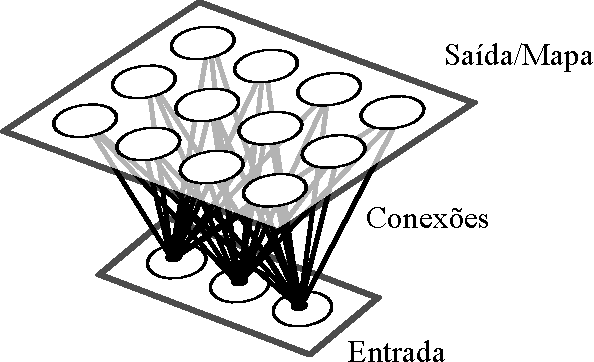
\includegraphics[height=5cm]{imagens/kohonen.pdf}
  \end{center}
  \caption{ Representação de uma rede de Kohonen. }
  \label{fig:kohonen}
\end{figure}

As redes de Kohonen possuem um algoritmo próprio de treinamento, dividido em
três etapas; na primeira, chamado de processo competitivo, uma determinada entrada
ativa apenas um neurônio da malha; na segunda, chamado de processo cooperativo,
o neurônio escolhido estabelece uma vizinhança de neurônios que serão ajustados
para, junto com ele, identificar padrões semelhantes ao que foi apresentado; e
por fim, na terceira etapa, chamada de processo adaptativo, os pesos são
atualizados com base no neurônio vencedor e na vizinhança topológica. Este
algoritmo de treinamento é dito não supervisionado, pois não depende de um
par \textit{(entrada, saída esperada)}, já que a própria rede estabelece como
será a configuração dos resultados, o processo de auto organização da rede.

\section{Características gerais de uma rede neural de Kohonen}\label{sec:caracteristicas_rede_kohonen}

Esta seção irá apresentar mais detalhadamente como é a configuração de uma rede
de Kohonen e seu algoritmo de treinamento.

\subsection{Topologia de uma rede de Kohonen}

Como dito anteriormente, a rede de Kohonen apresenta apenas duas camadas de
neurônios, a camada de entrada e a camada de saída. A camada de entrada deve
possuir tantos neurônios quanto forem à quantidade de elementos do padrão de
entrada. A camada de saída é uma grade de geometria livre, geralmente
retangular, de neurônios que não estão ligados entre si, mas estão, cada um,
ligados a todos os neurônios da camada de entrada. As conexões apresentam pesos
para escalar o sinal enviado. O esquema conceitual de uma rede de Kohonen é
demonstrado na Figura \ref{fig:kohonen_esquema}:

\begin{figure}[H]
  \begin{center}
    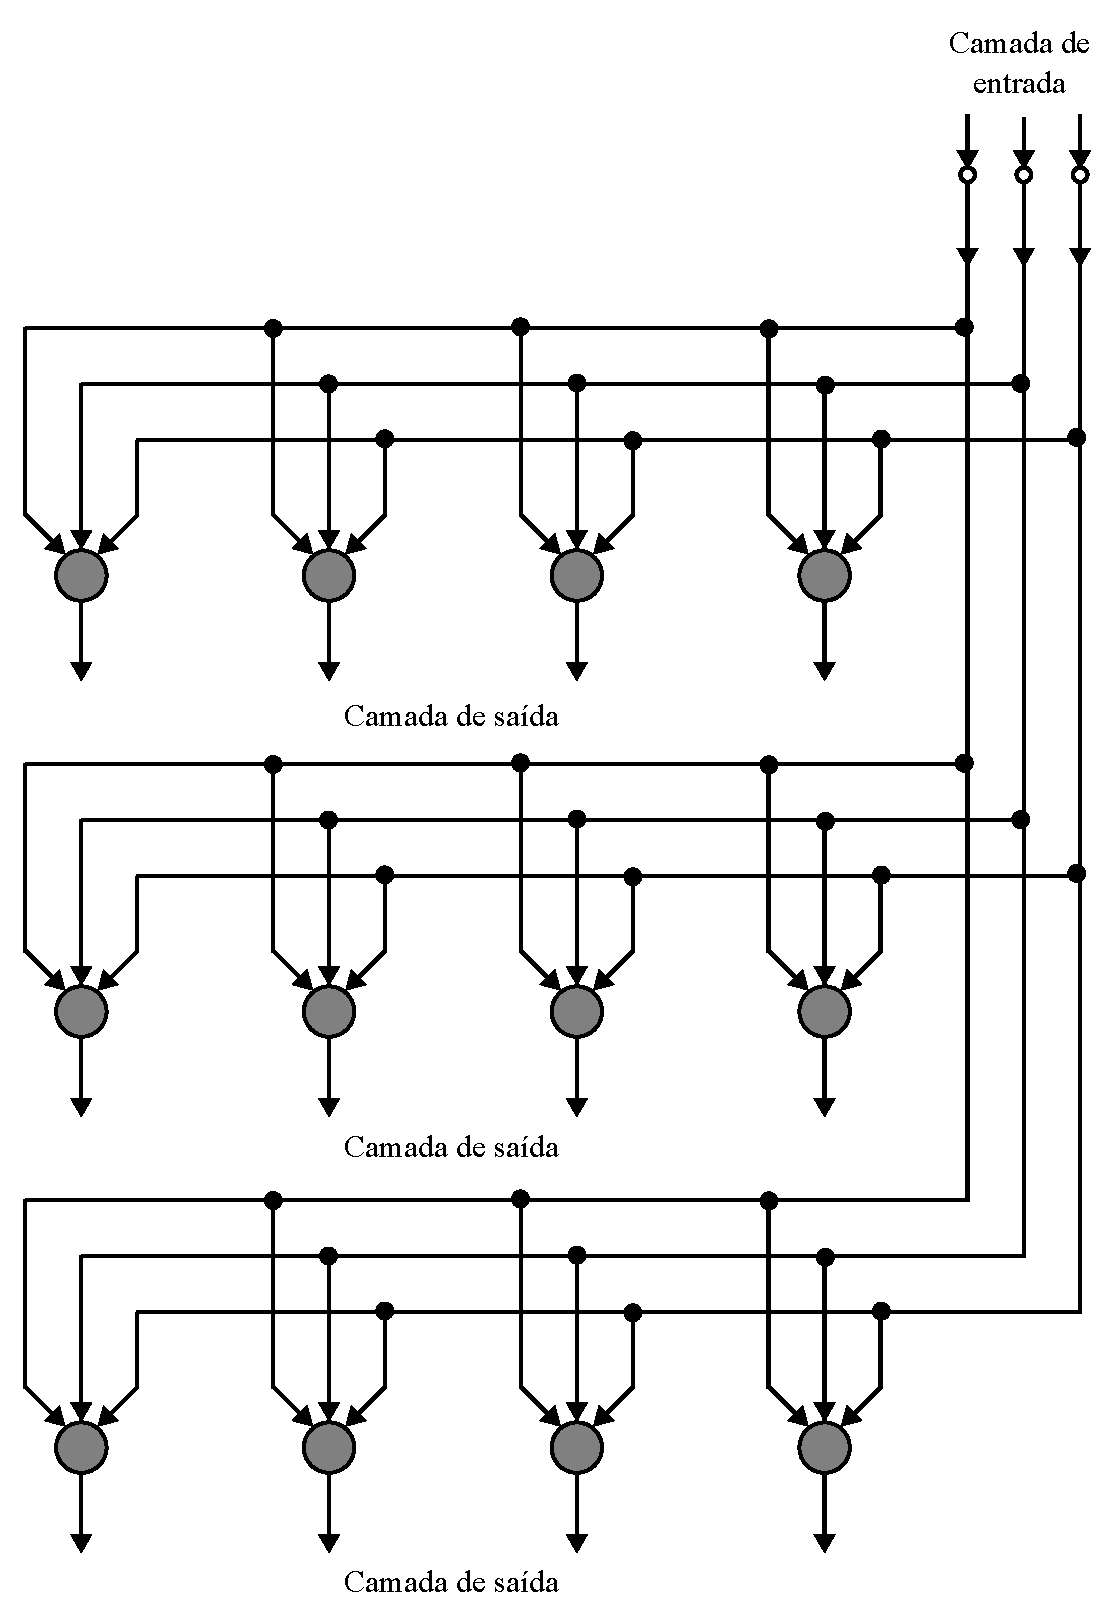
\includegraphics[height=18cm]{imagens/rede_detalhada.pdf}
  \end{center}
  \caption{ Esquema detalhado de uma rede de Kohonen. }
  \label{fig:kohonen_esquema}
\end{figure}

\subsection{Treinamento da rede}

O treinamento requer que os pesos sinápticos sejam iniciados com valores bem
pequenos, para que a rede não apresente inicialmente nenhuma configuração. Três
processos são executados para cada entrada do conjunto de treinamento, o
processo competitivo, o processo cooperativo e o processo adaptativo.

\subsubsection{Processo competitivo}

Quando uma entrada $ x = \left[x_1, x_2, ..., x_n\right]^T $ é apresentado à
rede, o neurônio da grade que melhor responder a este padrão será ativado, este
neurônio é dito vencedor, e será recompensado ajustando-se seus componentes
para mais próximo do vetor de entrada.

O critério escolhido para determinar o neurônio vencedor é a distância
euclidiana entre o vetor de entradas e o vetor de pesos das sinapses do
neurônio, como indicado na equação \ref{eq:dit_ecl}:

\begin{equation}\label{eq:dit_ecl}
d_i(t) = \sqrt{\sum_{j = 1}^N \left( x_j(t) - w_{ij}(t) \right)^2}
\end{equation}

Onde:

\begin{itemize}
\item $ d_i(t) $ é a distância euclidiana entre o vetor de pesos do
neurônio $ i $ e o vetor de entradas na iteração $ t $;
\item $ i $ é o índice do neurônio da grade;
\item $ j $ é o índice do neurônio de entrada;
\item $ N $ é o número de entradas;
\item $ x_j(t) $ é o sinal de entrada na entrada $ j $ na iteração $ t $;
\item $ w_{ij}(t) $ é o valor do peso sináptico entre o neurônio de
entrada $ j $ e o neurônio da grade $ i $ na iteração $ t $.
\end{itemize}

\subsubsection{Processo cooperativo}

Estudos biológicos indicam que ao ser excitado, um neurônio estimula seus
vizinhos topológicos, de forma que quanto mais próximo um neurônio está do
neurônio ativo, mais excitado pelo estímulo do neurônio ativo ele é. O processo
cooperativo busca simular este mecanismo biológico.

Em termos matemáticos, o que se deseja é um parâmetro $ h_{ik} $ , dito
\textit{vizinhança topológica}, que indica o gral de cooperação entre o
neurônio vencedor $ i $ e o seu vizinho $ k $, que deve ser simétrico em relação
ao neurônio $ k $ e deve decrescer constantemente com o aumento da
distância $ l_{ik} $ , até que $ \lim\limits_{ l_{ik} \to \infty } h_{ik} = 0 $ .
A função gaussiana \ref{eq:gauss} atende a estas duas exigências:

\begin{equation}\label{eq:gauss}
h_{ik} = e^{ \left( \frac{ l_{ik}^2 }{ 2 \sigma^2 } \right) }
\end{equation}

O parâmetro $ \sigma $ é denominado \textit{largura efetiva da vizinhança},
e deve diminuir a cada iteração, indicando uma tendência de especialização da
rede. Neste trabalho o parâmetro $ \sigma $ é a equação \ref{eq:leg_eft}:

\begin{equation}\label{eq:leg_eft}
\sigma(t) = \sigma_0 e^{ t / \tau_l }
\end{equation}

Onde:

\begin{itemize}
\item $ \sigma_0 $ é o valor inicial de $ \sigma $;
\item $ t $ é a iteração atual;
\item $ \tau_l $ é uma constante de tempo.
\end{itemize}

\subsubsection{Processo adaptativo}

O processo adaptativo atualiza os pesos sinápticos a cada iteração, levando em
consideração o neurônio vencedor e a vizinhança topológica. O ajuste dos pesos
deve decrescer com o tempo, para evitar que novos dados comprometam seriamente
o conhecimento já adquirido, substituindo padrões já estabelecidos por novos.
Algo semelhante ocorre com o cérebro humano, ao decorrer do envelhecimento o
aprendizado vai se tornando mais difícil.

O ajuste $ \Delta w_{ij} $ que a sinapse entre o neurônio de entrada $ i $ e
um neurônio da malha $ j $ deve sofrer é expresso pela equação \ref{eq:ajus}:

\begin{equation}\label{eq:ajus}
\Delta w_{ij} = \eta(t) h_{ik}(t) (x_j - w_{ij})
\end{equation}

Onde $ h_{ik}(t) $ é o parâmetro vizinhança topológica na iteração $ t $ ,
referente ao neurônio vencedor $ k $ . O
parâmetro \textit{taxa de aprendizagem} $ \eta(t) $ é definido pela
expressão \ref{eq:tx_aprd}:

\begin{equation}\label{eq:tx_aprd}
  \eta(t) = \eta_0 e^{ t / \tau_l }, \eta_0 \in [0, 1]
\end{equation}

Onde $ \tau_l $ é uma constante de tempo.

\subsubsection{Algoritmo geral de treinamento}

O algoritmo \ref{alg:trei_khn} resume as três etapas anteriores e descreve
todo o processo de treinamento de uma rede de Kohonen:
%\clearpage

\begin{algorithm}[H]
\caption{Treinamento de uma rede de Kohonen}\label{alg:trei_khn}
\SetAlgoRefName{alg:trei_khn}
\Entrada{$ \sigma_0 $ , $ \tau_l $ , $ \eta_0 $ e o valor do \textit{erro} }
\Inicio{
  \Repita{distâncias auclidianas $ \le $ erro}{
    Calcular a \textit{largura efetiva} $ \sigma(t) $\;
    Calcular a \textit{vizinhança topológica} $ h $\;
    Calcular a \textit{taxa de aprendizado} $ \eta(t) $\;
    \ParaCada{conexão}{
      Calcular $ \Delta w $\;
      Ajustar o arco\;
    }
  }
}
\end{algorithm}

\section{Normalização dos dados de entrada da rede}\label{sec:entrada_rede}

Neste ponto já deve estar claro que a entrada da rede será o conjunto dos sete
momentos invariantes. Os momentos serão utilizados tanto na etapa de treinamento
quanto na classificação das imagens propriamente dita. Contudo, da forma como os
momentos são calculados ainda é necessário que eles passem por uma normalização
com o propósito de equalizar os valores dos momentos segundo sua real
contribuição para caracterização das imagens, isto é, para cada um dos conjuntos
de momentos, sete no total, um ajuste é feito sobre cada valor conforme o gral de
variação dos dados, isto porque, se os valores de um conjunto são muito
parecidos, pode-se concluir que este conjunto não é uma característica forte
para distinguir as diferentes classes de imagens, então deve ter uma influência
menor na classificação que os demais com alta variação dos dados.

A normalização também ajusta a faixa dos valores dos momentos. Dado que os
valores geralmente são bem pequenos, a normalização amplifica proporcionalmente
todos eles e evita problemas envolvendo operações computacionais com números
muito próximos de zero.

Sendo $ M $ a matriz com os valores originais dos momentos, na forma:

\begin{equation}\label{eq:momentos_matriz}
  M = \left[
    \begin{array}{cccc}
        m_{11} & m_{12} & \hdots & m_{17} \\
        m_{21} & m_{22} & \hdots & m_{27} \\
        \vdots & \vdots & \ddots & \vdots \\
        m_{n1} & m_{n2} & \hdots & m_{n7} \\
    \end{array}
  \right]
\end{equation}

A tranformação $ N(M) $ que normaliza todos dos elementos de $ M $ é dada por:

\begin{equation}\label{eq:momentos_transformacao}
  N_{ij} = \frac{m_{ij} - \overline{H}_j}{\sigma_j}
\end{equation}

Onde:

\begin{itemize}
\item $ m_{ij} $ é o momento da linha $ i $ coluna $ j $ de $ M $;
\item $ \overline{H}_j $ é a média de todos os elementos da coluna $ j $ de $ M $;
\item $ \sigma_j $ é desvio padrão $ \sqrt{\frac{\sum_{i=1}^n (m_{ij} - \overline{H}_j)^2}{n - 1}} $
      dos elementos da coluna $ j $.
\end{itemize}

Por fim, cada linha da matriz $ N $ é enviada para rede tanto na etapa do treinamento
quanto para classificação da imagem.

\section{A rede neural de Kohonen e o agrupamento das imagens}\label{sec:rede_kohonen_imagens}

O conjunto dos pesos sinápticos é o resultado obtido pelo processo de
treinamento, eles determinarão a posição de cada imagem no mapa, deste modo, os
momentos normalizados de cada imagem devem ser apresentados a rede numa segunda
vez para serem classificados.

Contudo, a posição das imagens apenas não indica a que classe pertencem, e na
verdade, até agora as classes ainda não foram determinadas, para isso é
necessário a adição de outros formalismos que através das posições das imagens
e dos pesos sinápticos identifiquem as classes e rotule cada imagem para uma
delas.

Nas subseções abaixo serão apresentados dois conceitos que determinam as classes
de uma rede de Kohonen, a matriz de distâncias unificadas e a transformada de
\textit{watershed}.

\subsection{Matriz de distâncias unificadas}\label{sec:u_matriz}

Tendo executado o treinamento da rede de Kohonen, pode parecer que a distância
euclidiana entre os elementos mapeados é o único parâmetro para a identificação
das classes, contudo, existe também uma distância do vetor de entrada para cada
posição do mapa, isto implica que também há uma outra distância entre os
neurônios além da distância euclidiana, uma distância que representa o grau de
dificuldade de se classificar uma elemento, no caso as imagens, em outra posição
diferente da que naturalmente lhe seria atribuída. Isto faz muita diferença
porque, mesmo sendo necessário que as classes tenham elementos adjacentes, esta
não é condição suficiente para identificação dos grupos, é possível que
dois elementos próximos pertençam a duas classes distintas, para isto basta
que a dificuldade de se classificar um desses elementos na posição do outro seja
superior a um limite estipulado.

Fazendo uma análise visual destas considerações, seria como se o mapa possuísse
campos de atração, formando vales e picos, sendo os vales as classes e os picos
os seus limites, ou fronteiras, como indica a Figura \ref{fig:mapa_x_umatriz}.

\begin{figure}[H]
  \begin{center}
    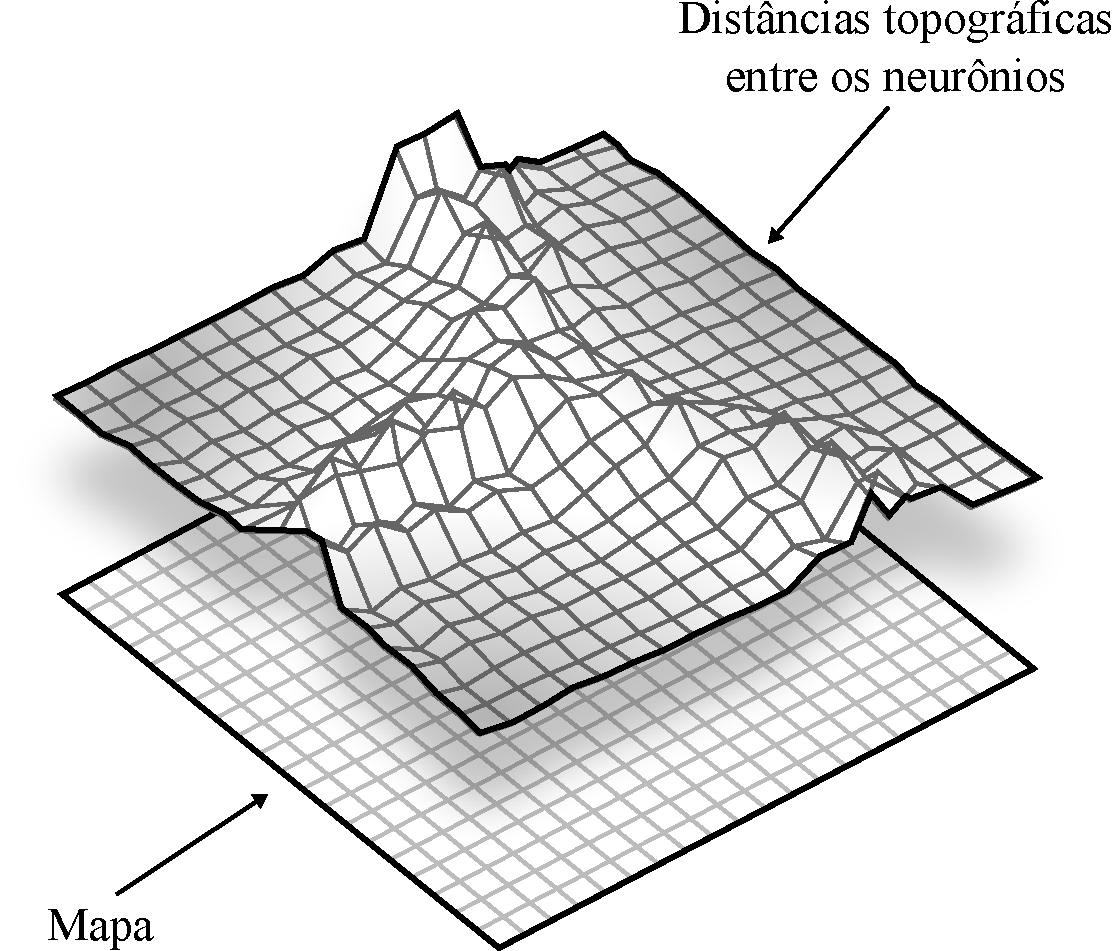
\includegraphics[height=8cm]{imagens/mapa_x_umatriz.pdf}
  \end{center}
  \caption{ Representação da malha de distâncias topográficas entre os neurônios }
  \label{fig:mapa_x_umatriz}
\end{figure}

O método denominado matriz de distâncias unificadas, ou simplesmente U-Matriz,
tem o objetivo de identificar estas relações topológicas, definindo uma função
tridimensional onde cada ponto do plano apresenta um valor de distância entre
neurônios adjacentes, de modo que valores baixos correspondem a neurônios
vizinhos semelhantes e valores altos correspondem a neurônios vizinhos
diferentes. Em termos matemáticos, regiões com baixos valores do gradiente,
vales, são classes de neurônios especializados em padrões similares e regiões
com valores altos correspondem a fronteiras entre as classes.

Considere o mapa retangular discreto limitado de tamanho $ N \times M $, para cada
neurônio $ p $ da camada de saída existe, na U-matriz, três distâncias, $ d_x $,
$ d_y $ e  $ d_{xy} $, em relação a seus vizinhos, como indicado na Figura \ref{fig:dxdydxy}.

\begin{figure}[H]
  \begin{center}
    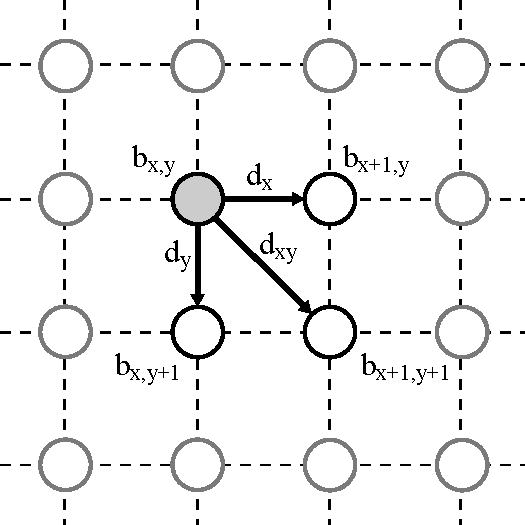
\includegraphics[height=6cm]{imagens/dxdydxy.pdf}
  \end{center}
  \caption{ Distâncias $ d_x $, $ d_y $ e $ d_{xy} $ entre o neurônio $ b_{x,y} $
    e seus visinhos. }
  \label{fig:dxdydxy}
\end{figure}

Os valores de $ d_x $, $ d_y $ e $ d_{xy} $ são calculados da seguinte maneira:

\begin{subequations}\label{eq:dxdydxy}
\begin{align}
  d_x(x, y) = \sqrt{\sum_i{ \left( w_{i(x,y)} - w_{i(x + 1, y)} \right)^2 }}\\
  d_y(x, y) = \sqrt{\sum_i{ \left( w_{i(x,y)} - w_{i(x, y + 1)} \right)^2 }}\\
  d_y(x, y) = \frac{1}{2\sqrt{2}}\sqrt{\sum_i{ \left( w_{i(x,y)} - w_{i(x + 1, y + 1)} \right)^2 } + \sum_i{ \left( w_{i(x,y + 1)} - w_{i(x + 1, y)} \right)^2 } }
\end{align}
\end{subequations}

Estes valores são inseridos em uma matriz de tamanho $ (N-1) \times (M-1) $ de acordo
com a seguinte tabela:

\begin{center}
\begin{tabular}{|c|c|c|}
\hline
  \textbf{i} & \textbf{j} & \textbf{$ U_{ij} $} \\
\hline
\hline
  $ 2x + 1 $ &     $ 2y $ & $ d_x(x,y) $    \\
\hline
      $ 2x $ & $ 2y + 1 $ & $ d_y(x,y) $    \\
\hline
  $ 2x + 1 $ & $ 2y + 1 $ & $ d_{xy}(x,y) $ \\
\hline
      $ 2x $ &     $ 2y $ & $ d_u(x,y) $    \\
\hline
\end{tabular}
\end{center}

Sendo $ c = [c_1, c_2, ..., c_k ] $ o vetor ordenado de elementos circunvizinhos
com cardinalidade $ k $, ainda levando em consideração um mapa retangular, o
cálculo de $ d_u $ é obtido pela mediana dos valores circunvizinhos,
do seguinte modo:

\begin{equation}\label{eq:du}
  d_u(x,y) = \left\{
    \begin{array}{rc}
                          c_{(k + 1)/2}, & \mbox{se $ k $ for ímpar} \\
      \frac{c_{k/2} + c_{(k + 1)/2}}{2}, & \mbox{se $ k $ for par}
    \end{array}
  \right.
\end{equation}

Deste modo, a organização da U-Matriz é ilustrada pela
Figura \ref{fig:mapa_umatriz}:

\begin{figure}[H]
  \begin{center}
    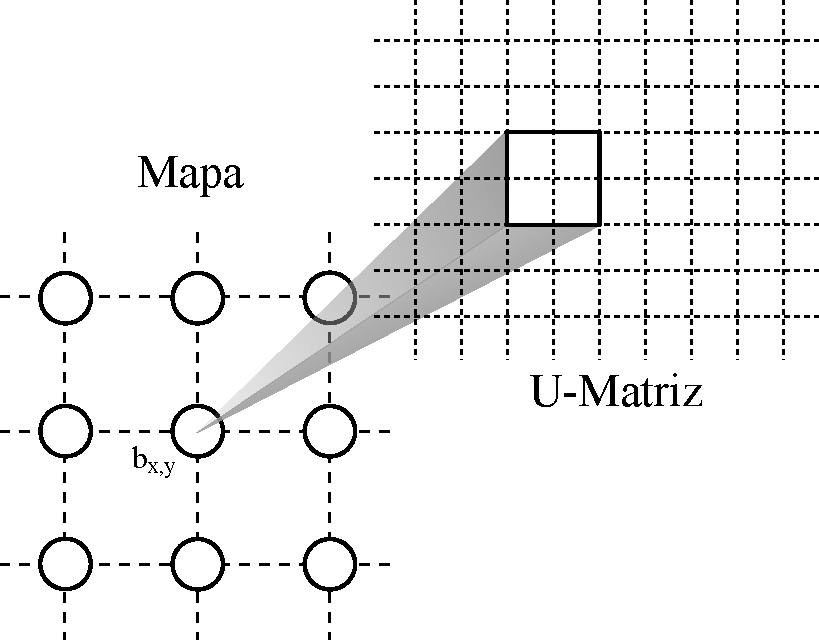
\includegraphics[height=6cm]{imagens/mapa_umatriz.pdf}
  \end{center}
  \caption{ Organização da U-Matriz em relação a grade de neurônios. }
  \label{fig:mapa_umatriz}
\end{figure}

\subsection{Transformada \textit{watershed} para rotulação automática
da U-Matriz}\label{sec:watershed}

A transformada de \textit{watershed} estabelece as regiões e fronteiras das
classes com base na U-matriz, faz isso apoiada no conceito intuitivo de
inundação, vales e diques, da seguinte maneira:

Como visto na Seção \ref{sec:u_matriz}, a U-matriz pode ser interpretada como
uma superfície que contem vales e montanhas, considerando uma inundação, a água
escorre pelas montanhas até os vales, que se inundam com o tempo, formando
bacias. Em um determinado momento certas bacias tenderão a se unir, esta união
é impedida pela “construção” de diques entre as regiões de fronteira. Ao fim do
processo, ou seja, quando a água chegar ao nível da maior montanha, os diques
formarão as fronteiras e as bacias formarão as classes. A Figura
\ref{fig:tempo_inundacao} Ilustra esse processo:

\begin{figure}[H]
  \begin{center}
    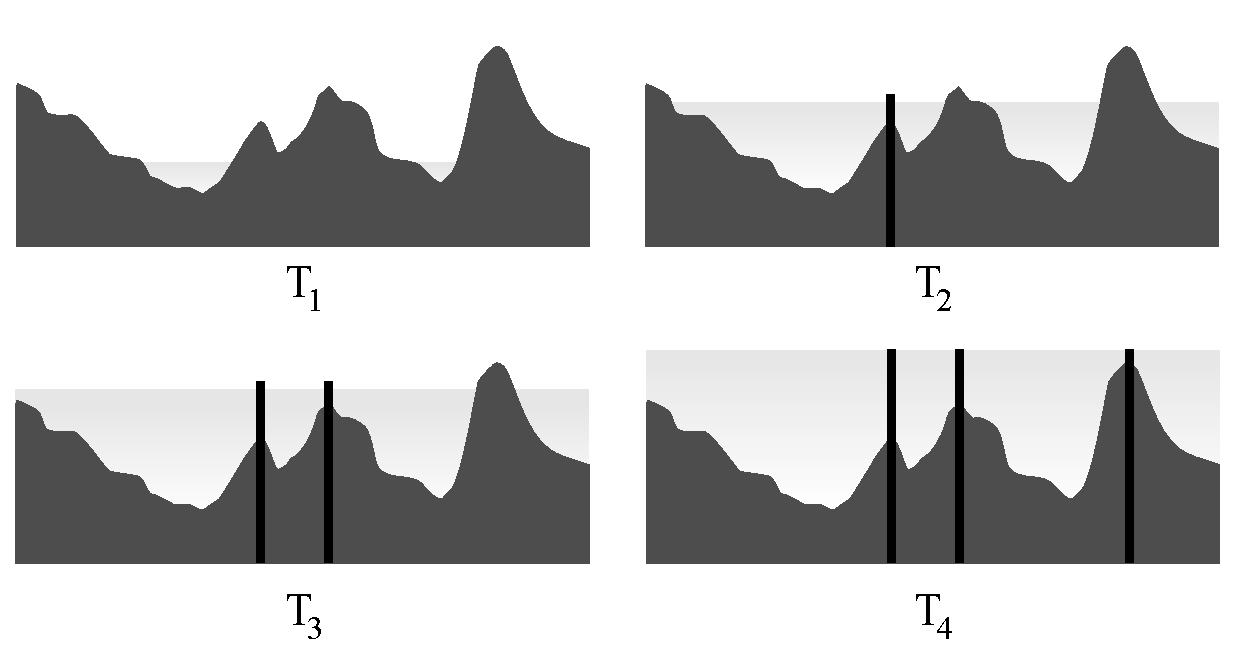
\includegraphics[height=8cm]{imagens/diques_tempo.pdf}
  \end{center}
  \caption{ Esquema conceitual do funcionamento da transformada de
    \textit{watershed} durante quatro períodos onde a “inundação” vai
    tomando os “vales”. }
  \label{fig:tempo_inundacao}
\end{figure}

Uma definição formal da transformada de \textit{watershed} passa pela
consideração de dois períodos, isto é, pelo processo de expansão das bacias, em
outros termos, pela elevação de um nível $ h $ para $ h + 1 $.

Uma bacia associada a um mínimo $ m $ é denominada de $ B(m) $, os pontos dessa
bacia que possuem altitude menor ou igual a $ h $ são denominados $ B_h(m) $,
isto é:

\begin{equation}\label{eq:watershed_bm}
  B_h(m) = \{ p \in B(m) | f(p) \le h \}
\end{equation}

O subconjunto de todas as bacias que possuem pontos com altitude menor ou igual
a $ h $ é denominado $ X(h) $, formalmente:

\begin{equation}\label{eq:watershed_xh}
  X(h) = \bigcup_i B_h(m_i)
\end{equation}

Junto a esses conceitos fundamentais, o conjunto de todas os pontos que
pertencem ao mínimo regional $ m_h $ de elevação $ h $ é denominado $ R_{min_h}(f)$.
Esta região será definida posteiormente ainda nesta seção.

Considerando que os primeiros pontos a serem inundados são os pontos mínimos
$ h_{min} $, podemos aplicar a Equação \ref{eq:watershed_xh} da forma:

\begin{equation}\label{eq:watershed_xhmin}
  X(h_{min}) = R_{min_{h_{min}}}(f) = T_{h_{min}}(f)
\end{equation}

Onde $ T $ obedece a relação:

\begin{equation}\label{eq:watershed_t}
  T_h(f(x)) = \left\{
    \begin{array}{rc}
      x, & \mbox{se $ h \le f(x) $} \\
      0, & \mbox{qualquer outro}
    \end{array}
  \right.
\end{equation}

Utilizando $ h_{min} $ como ponto de partida, agora é necessário avançar para o
estágio onde o nível sobe uma unidade, ou seja, para $ h_{min + 1} $.
Neste ponto três situações podem ocorrer, isoladas ou simultaneamente, 1)
um novo mínimo será encontrado no ponto $ h_{min + 1} $ e formará uma
nova bacia, 2) ocorrerá uma expansão da bacia da região cujo mínimo é $ h_{min} $ e
3) duas ou mais bácias distintas de nível $ h_{min} $ estão se
expandindo e se encontrarão juntas. Estas três situações são ilustradas na
Figura \ref{fig:niveis}:

\begin{figure}[H]
  \begin{center}
    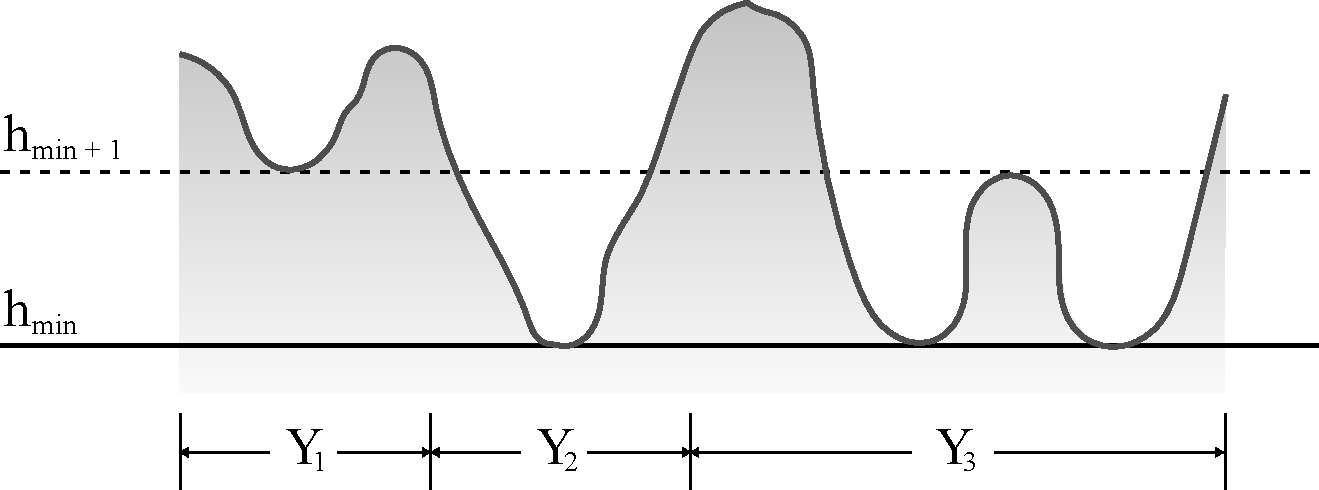
\includegraphics[height=5cm]{imagens/niveis.pdf}
  \end{center}
  \caption{ As três possíveis sutuações na passagem do nível $ h_{min} $ para
    $ h_{min + 1} $ . }
  \label{fig:niveis}
\end{figure}

1) $ Y_1 \cap X_{h_{min}} = \emptyset $: Nenhuma bacia foi formada, o que ocorrerá
apenas no próximo avanço de nível. Neste caso, vale a relação:

\begin{equation}\label{eq:watershed_caso1}
  \forall p \in Y_1 \left\{
    \begin{array}{rc}
      p \notin X_{h_{min}} \Rightarrow & f(p) \ge h_{min} + 1 \\
                 p \in Y_1 \Rightarrow & f(p) \le h_{max}
    \end{array}
  \right.
\end{equation}

2) $ Y_2 \cap X_{h_{min}} \neq \emptyset $ e é conectado: Neste caso a inundação já atingiu o
mínimo de $ Y_2 $ e o processo se encaminha numa expansão da bacia, o que pode
ser descrito como:

\begin{equation}\label{eq:watershed_caso21}
  Y_2 = B_{h_{min} + 1}(Y_2 \cap X_{h_{min}}) = Z_{Y_2}(Y_2 \cap X_{h_{min}})
\end{equation}

Onde $ Z_{Y_2}(Y_2 \cap X_{h_{min}}) $ é a zona de influência geodésica de
$ Y_2 \cap X_{h_{min}} $ contida em $ Y_2 $. Esta zona de influência
geodésica $ Z_A(K_i) $ de um componente conectado $ K_i $ dentro de um conjunto $ A $
é o lugar geométricos dos pontos
de $ A $ que a distância geodésica para $ K_i $ é a menor que a distância
geodésica para qualquer outro ponto de $ A $, em outros termos:

\begin{equation}\label{eq:watershed_caso22}
  Z_A(K_i) = \{ p \in A, \forall j \in [1, N] - \{ i \}, d_A(p, K_i) < d_A(p, K_j) \}
\end{equation}

Onde a distância geodésica $ d_A(p, q) $ entre dois pontos $ p $ e $ q $
pertencentes a $ A $ é o menor caminho entre todos os caminhos possíveis de
pontos, também pertencentes a $ A $, que ligam $ p $ e $ q $.

3) $ Y_3 \cap X_{h_{min}} \neq \emptyset $ e não é conectado: Neste caso $ Y_3 $
contém dois ou mais mínimos e eles estão expandindo juntos, denotados de
$ M_1, M_2, …, M_k $. Sendo $ M_i $ uma destas regiões a melhor aproximação
para $ B_{h_{min + 1}}(M_i) $ corresponde a zona de influência geodésica de $ M_i $
dentro de $ Y_3(M_Y)$:

\begin{equation}\label{eq:watershed_caso3}
  B_{h_{min + 1}}(M_i) = Z_Y(M_i)
\end{equation}

Como em 2) e 3) são bacias que estão em expansão, podemos definir estas regiões em termos
de uma única zona de influência geodésica $ X_{h_{min}} $, deste modo
$ X_{h_{min + 1}} $ é definido como a união destas zonas de influência geodésicas
onde os mínimos regionais foram os mais recentemente descobertos,
formulado em termos de uma recursão:

\begin{equation}\label{eq:watershed_recursao}
  \left\{
    \begin{array}{l}
      X_{h_{min}} = \bigcup_i h_{min_{i}} \in f \\
      X_{h + 1} = R_{min_{h + 1}}(f) \cup Z_{T_{t \le {h + 1}(f)}}(X_h)
    \end{array}
  \right.
\end{equation}

Por fim, o conjunto de bacias encontradas na U-matriz representam as classes e
servirão para rotular as imagens, para cada mínimo local haverá uma bacia e com
isso uma classe. Como o conjunto de mínimos locais pode ser grande, existe então
a chance de uma sobre segmentação da U-matriz, por isso é conveniente restringir
a quantidade de mínimos locais, no caso, os mínimos locais que geram bacias
com regiões muito pequenas, logo, é comum a utilização de filtros gaussianos
sobre a U-matriz antes de se aplicar a transformada de \textit{watershed} para
regularizá-la.

\section{Resumo do processo de classificação das imagens e do \textit{clustering}
como um todo}\label{sec:resumo_clustering}

Agora que foram apresentados todos as teorias utilizadas nesta técnica de
clustering, bem como suas devidas justificativas, é conveniente resumir todo o
processo de um ponto de vista macro, enumerando e explicando brevemente cada uma
das etapas, vejamos:

O dado inicial é o conjunto de imagens que serão classificadas, a primeira etapa
consiste em tratá-las e calcular os mementos invariantes de cada uma delas, como
descrito no Capítulo 2. O conjunto dos momentos formam a matriz $ M $ e passa
pela etapa de normalização como descrito na Seção \ref{sec:entrada_rede}. Os
momentos normalizados são um a um enviados para rede de Kohonen com o objetivo
de treiná-la, este treinamento ocorre como apresentado na
Seção \ref{sec:caracteristicas_rede_kohonen} e é dividido pelas subetapas de
competição, cooperação e adaptação, que também são executados em sequência para
cada momento individualmente. O envio dos momentos a rede dura o tempo
necessário para que o erro seja tolerável, como descrito pelo
Algoritmo \ref{alg:trei_khn}, caso esta tolerância tenha sido atingida antes
que todas os momentos tenham sito processados, a rede é recriada com dimensões
maiores, neste caso diz-se que a rede saturou, isto é, atingiu o limite de
informação que pode aprender sem ter analisado todos os dados, deste modo a
criação de uma nova rede é inevitável e o treinamento deve ser reiniciado. O
resultado do treinamento são os pesos sinápticos devidamente ajustados para
mapear os momentos, e consecutivamente as imagens. Em seguida dois processos
paralelos tem incio, o primeiro é a verificação da posição no mapa que cada
imagem possui, e o segundo é a definição das classes dentro do mapa através do
cálculo da U-matriz e da transformada de \textit{watershed}. Havendo agora as
imagens mapeadas e as classes, por fim cada uma das imagens é rotulada com na
classe que sua posição está inserida.

A Figura \ref{fig:classificacao} resume visualmente todo o processo:

\begin{landscape}
  \begin{figure}[H]
    \begin{center}
      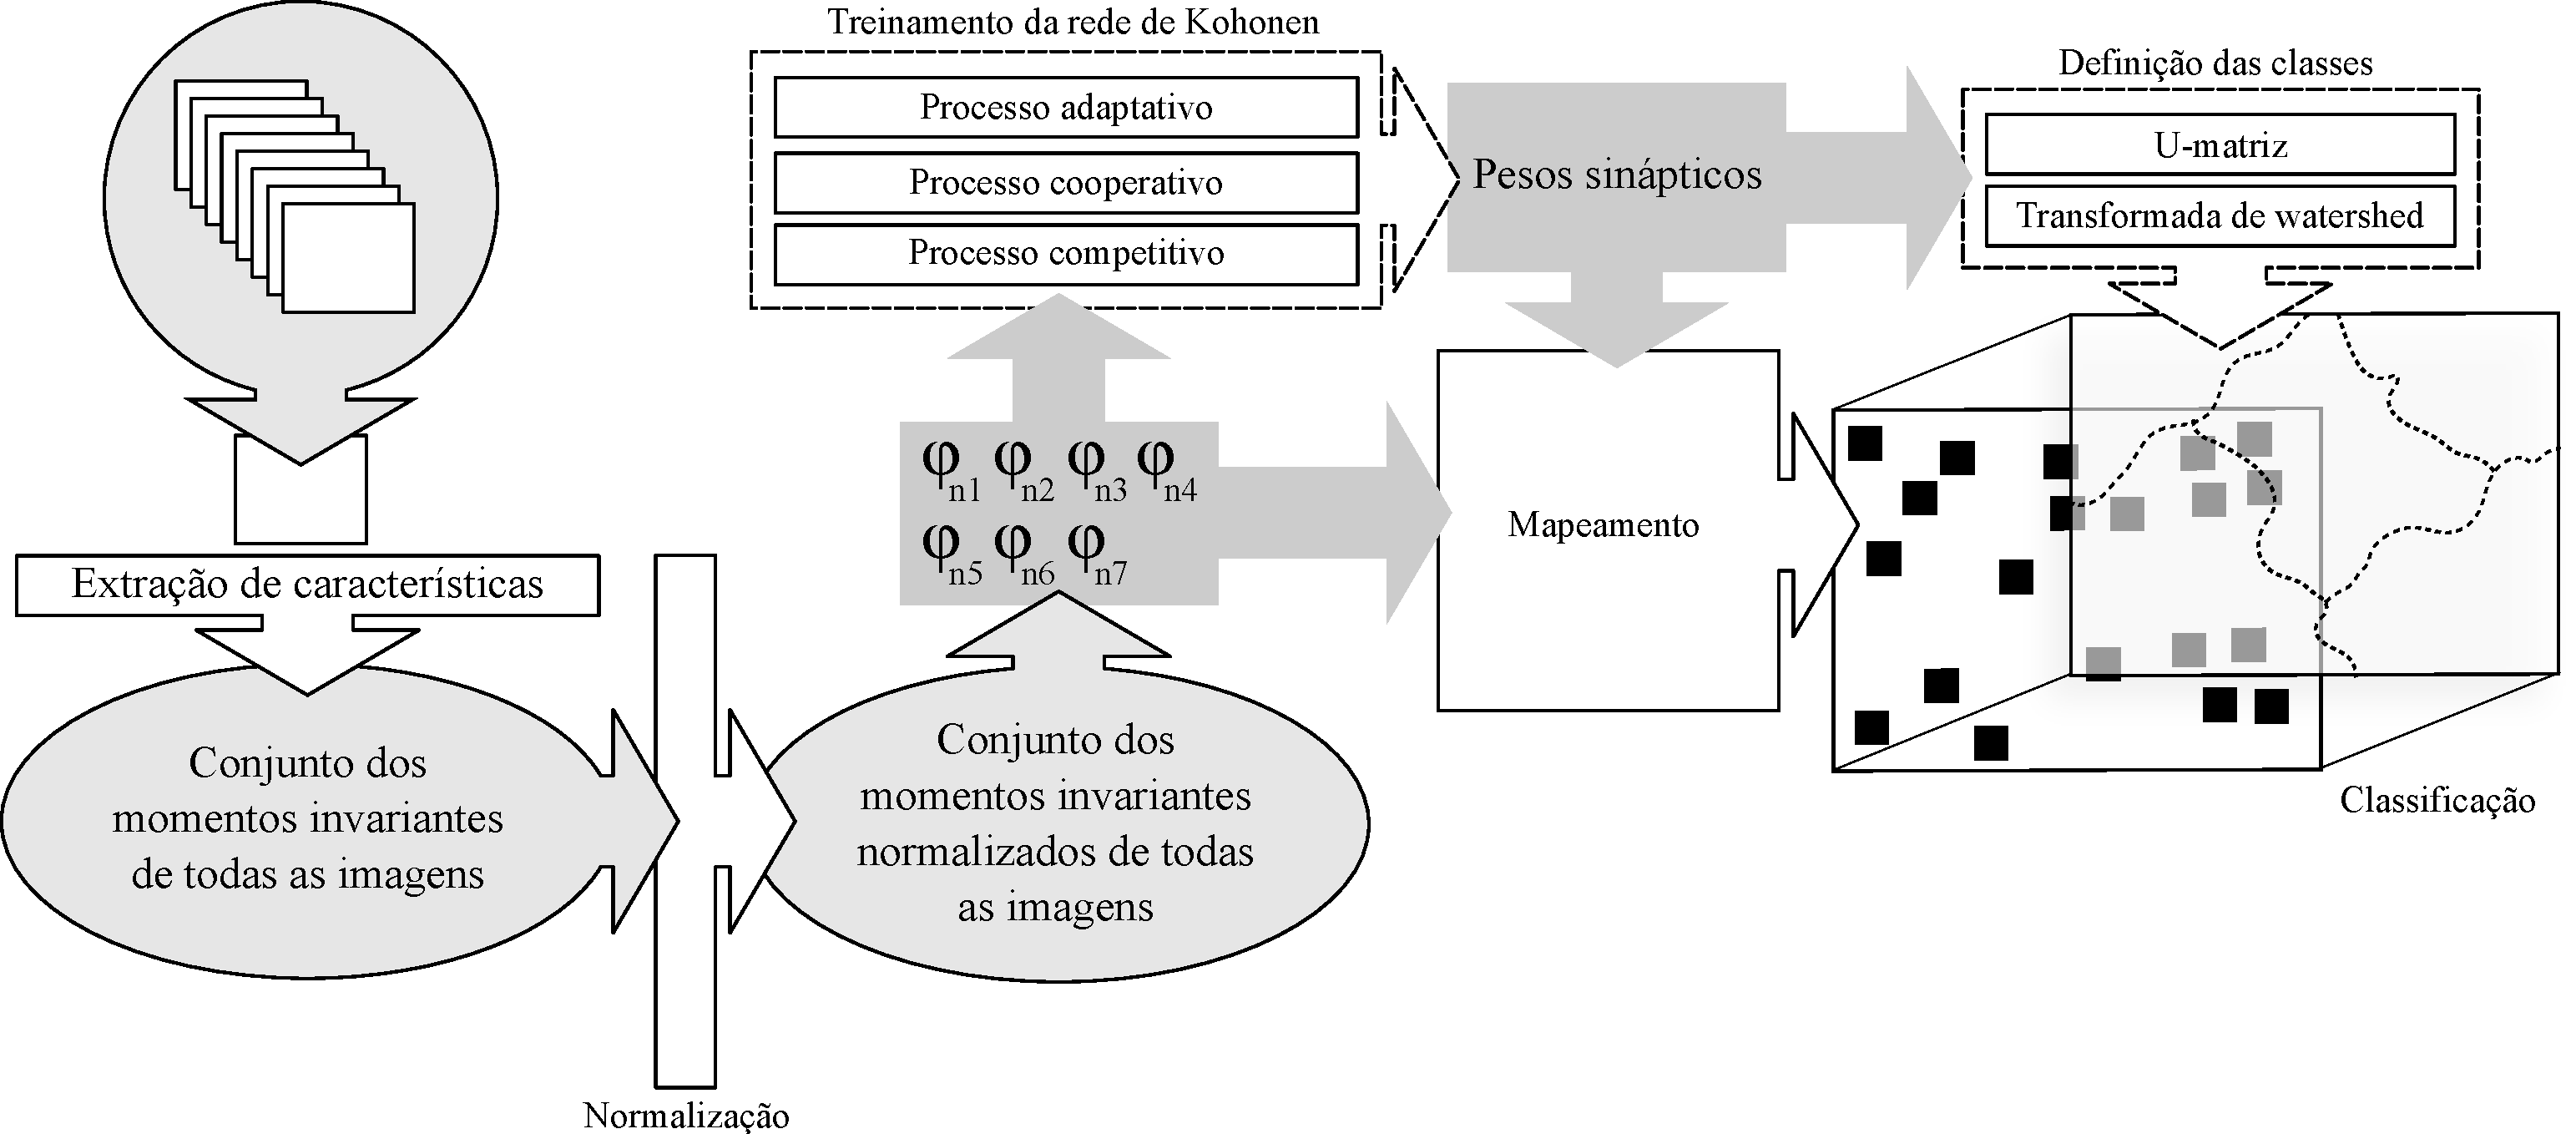
\includegraphics[height=10cm]{imagens/classificacao.pdf}
    \end{center}
    \caption{ Legenda. }
    \label{fig:classificacao}
  \end{figure}
\end{landscape}

\chapter{Testes empíricos e análise dos resultados}

TEXTO AQUI.

\section{Roteiro e fundamentação do teste proposto}

Este trabalho propõe como teste de validação para técnica de classificação
descrita nos capítulos anteriores um esquema simples de comparação de
expectativas, haverá um grupo de imagens previamente classificado por agentes
humanos, e outra classificação, para este mesmo grupo de imagens, gerada pela
técnica aqui proposta, deste modo, será possível efetuar a comparação entre a
expectativa, isto é, as classes que idealmente devem ser geradas, representadas
pela classificação humana das imagens, com as classes fornecidas pela técnica
baseada nas redes de Kohonen. As imagens utilizadas no teste são de tal modo
que sua classificação humana é auto-evidente, e deste modo, como será observado
na Seção \ref{sec:conjunto_de_imagens}, dificilmente serão alvo de alguma
contestação.

O objetivo do teste é avaliar a quantidade e a pertinência das classes, ou seja,
se o mesmo número de classes aparece em ambos as classificações e se as classes
geradas pelo método proposto possuem correspondência com as classes definidas
pelos agentes humanos, mais especificamente, se as imagens estão agrupadas pelo
método baseado nas redes de Kohonen do mesmo modo, ou de modo muito semelhante,
como foram agrupadas pelos agentes humanos.

\section{Especificação do conjunto de imagens e das classes de controle}
\label{sec:conjunto_de_imagens}

O conjunto de imagens utilizada para a execução do teste é o
\textit{Columbia Object Image Library} (COIL-100), um conjunto de 100
objetos em 7200 poses
diferentes. Destes 100, foram escolhidas 91 imagens de diferentes objetos para
compor o teste. Foram identificadas 15 classes para estas imagens, cada classe possui
imagens em poses com variações de translação, rotação e escala para o mesmo tipo
de objeto, afim de confrontar as premissas da Seção \ref{sec:momentos_desc} no
contexto do processo de classificação.

As classes identificadas foram nomeadas e apresentam as seguintes imagens:

\begin{table}[H]
  \centering
  \caption{Grupo A (animais de brinquedo).}
  \tabulinesep =_0.5em^0.5em
  \everyrow{\tabucline[0.4pt]-}
  \begin{tabu}{|ccccccc|}
    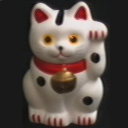
\includegraphics[width=0.1\textwidth,height=0.1\textwidth]{imagens/coil_100/animais_brinquedos/obj14__0.png} &
    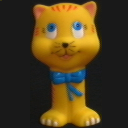
\includegraphics[width=0.1\textwidth,height=0.1\textwidth]{imagens/coil_100/animais_brinquedos/obj17__0.png} &
    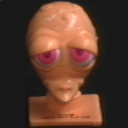
\includegraphics[width=0.1\textwidth,height=0.1\textwidth]{imagens/coil_100/animais_brinquedos/obj20__0.png} &
    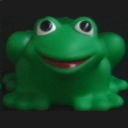
\includegraphics[width=0.1\textwidth,height=0.1\textwidth]{imagens/coil_100/animais_brinquedos/obj28__275.png} &
    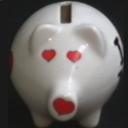
\includegraphics[width=0.1\linewidth,height=0.1\linewidth]{imagens/coil_100/animais_brinquedos/obj48__265.png} &
    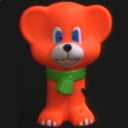
\includegraphics[width=0.1\linewidth,height=0.1\linewidth]{imagens/coil_100/animais_brinquedos/obj52__0.png} &
    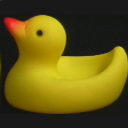
\includegraphics[width=0.1\linewidth,height=0.1\linewidth]{imagens/coil_100/animais_brinquedos/obj74__0.png}
    \\
    \scriptsize{obj01.jpg} & \scriptsize{obj02.jpg} & \scriptsize{obj03.jpg} &
    \scriptsize{obj04.jpg} & \scriptsize{obj05.jpg} & \scriptsize{obj06.jpg} &
    \scriptsize{obj07.jpg}
  \end{tabu}
\end{table}

\begin{table}[H]
  \centering
  \caption{Grupo B (barquinhos de brinquedo).}
  \tabulinesep =_0.5em^0.5em
  \everyrow{\tabucline[0.4pt]-}
  \begin{tabu}{|cccc|}
    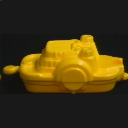
\includegraphics[width=0.1\textwidth,height=0.1\textwidth]{imagens/coil_100/barquinhos_brinquedos/obj3__0.png} &
    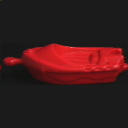
\includegraphics[width=0.1\textwidth,height=0.1\textwidth]{imagens/coil_100/barquinhos_brinquedos/obj38__0.png} &
    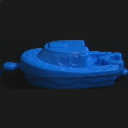
\includegraphics[width=0.1\textwidth,height=0.1\textwidth]{imagens/coil_100/barquinhos_brinquedos/obj42__0.png} &
    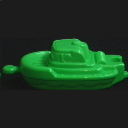
\includegraphics[width=0.1\textwidth,height=0.1\textwidth]{imagens/coil_100/barquinhos_brinquedos/obj78__0.png}
    \\
    \scriptsize{obj08.jpg} & \scriptsize{obj09.jpg} & \scriptsize{obj10.jpg} &
    \scriptsize{obj11.jpg}
  \end{tabu}
\end{table}

\begin{table}[H]
  \centering
  \caption{Grupo C (boias).}
  \tabulinesep =_0.5em^0.5em
  \everyrow{\tabucline[0.4pt]-}
  \begin{tabu}{|cc|}
    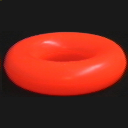
\includegraphics[width=0.1\textwidth,height=0.1\textwidth]{imagens/coil_100/boias/obj47__0.png} &
    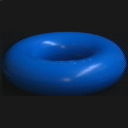
\includegraphics[width=0.1\textwidth,height=0.1\textwidth]{imagens/coil_100/boias/obj94__0.png}
    \\
    \scriptsize{obj12.jpg} & \scriptsize{obj13.jpg}
  \end{tabu}
\end{table}

\begin{table}[H]
  \centering
  \caption{Grupo D (caixas).}
  \tabulinesep =_0.5em^0.5em
  \everyrow{\tabucline[0.4pt]-}
  \begin{tabu}{|ccccc|}
    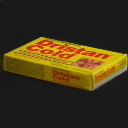
\includegraphics[width=0.1\textwidth,height=0.1\textwidth]{imagens/coil_100/caixas/obj1__35.png} &
    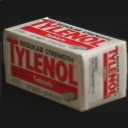
\includegraphics[width=0.1\textwidth,height=0.1\textwidth]{imagens/coil_100/caixas/obj31__45.png} &
    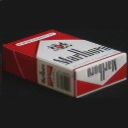
\includegraphics[width=0.1\textwidth,height=0.1\textwidth]{imagens/coil_100/caixas/obj46__45.png} &
    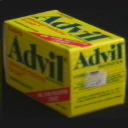
\includegraphics[width=0.1\textwidth,height=0.1\textwidth]{imagens/coil_100/caixas/obj54__55.png} &
    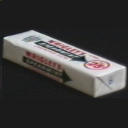
\includegraphics[width=0.1\textwidth,height=0.1\textwidth]{imagens/coil_100/caixas/obj67__50.png}
    \\
    \scriptsize{obj14.jpg} & \scriptsize{obj15.jpg} & \scriptsize{obj16.jpg} &
    \scriptsize{obj17.jpg} & \scriptsize{obj18.jpg}
    \\
    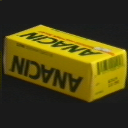
\includegraphics[width=0.1\textwidth,height=0.1\textwidth]{imagens/coil_100/caixas/obj79__45.png} &
    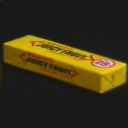
\includegraphics[width=0.1\textwidth,height=0.1\textwidth]{imagens/coil_100/caixas/obj84__45.png} &
    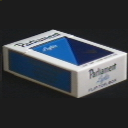
\includegraphics[width=0.1\textwidth,height=0.1\textwidth]{imagens/coil_100/caixas/obj96__45.png} &
    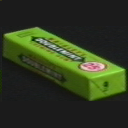
\includegraphics[width=0.1\textwidth,height=0.1\textwidth]{imagens/coil_100/caixas/obj98__55.png} &
    \\
    \scriptsize{obj19.jpg} & \scriptsize{obj20.jpg} & \scriptsize{obj21.jpg} &
    \scriptsize{obj22.jpg} &
  \end{tabu}
\end{table}

\begin{table}[H]
  \centering
  \caption{Grupo E (carrinhos de brinquedo).}
  \tabulinesep =_0.5em^0.5em
  \everyrow{\tabucline[0.4pt]-}
  \begin{tabu}{|cccccc|}
    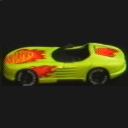
\includegraphics[width=0.1\textwidth,height=0.1\textwidth]{imagens/coil_100/carrinhos_brinquedos/obj6__0.png} &
    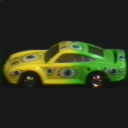
\includegraphics[width=0.1\textwidth,height=0.1\textwidth]{imagens/coil_100/carrinhos_brinquedos/obj8__0.png} &
    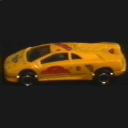
\includegraphics[width=0.1\textwidth,height=0.1\textwidth]{imagens/coil_100/carrinhos_brinquedos/obj15__0.png} &
    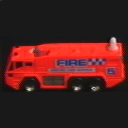
\includegraphics[width=0.1\textwidth,height=0.1\textwidth]{imagens/coil_100/carrinhos_brinquedos/obj19__0.png} &
    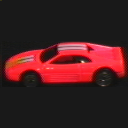
\includegraphics[width=0.1\textwidth,height=0.1\textwidth]{imagens/coil_100/carrinhos_brinquedos/obj23__0.png} &
    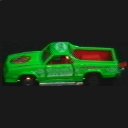
\includegraphics[width=0.1\textwidth,height=0.1\textwidth]{imagens/coil_100/carrinhos_brinquedos/obj27__0.png}
    \\
    \scriptsize{obj23.jpg} & \scriptsize{obj24.jpg} & \scriptsize{obj25.jpg} &
    \scriptsize{obj26.jpg} & \scriptsize{obj27.jpg} & \scriptsize{28obj.jpg}
    \\
    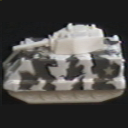
\includegraphics[width=0.1\textwidth,height=0.1\textwidth]{imagens/coil_100/carrinhos_brinquedos/obj37__0.png} &
    \includegraphics[width=0.1\textwidth,height=0.1\textwidth]{imagens/coil_100/carrinhos_brinquedos/obj69__0.png} &
    \includegraphics[width=0.1\textwidth,height=0.1\textwidth]{imagens/coil_100/carrinhos_brinquedos/obj76__0.png} &
    \includegraphics[width=0.1\textwidth,height=0.1\textwidth]{imagens/coil_100/carrinhos_brinquedos/obj91__0.png} &
    \includegraphics[width=0.1\textwidth,height=0.1\textwidth]{imagens/coil_100/carrinhos_brinquedos/obj100__0.png} &
    \\
    \scriptsize{obj29.jpg} & \scriptsize{obj30.jpg} & \scriptsize{obj31.jpg} &
    \scriptsize{obj32.jpg} & \scriptsize{obj33.jpg} &
  \end{tabu}
\end{table}

\begin{table}[H]
  \centering
  \caption{Grupo F (chícaras).}
  \tabulinesep =_0.5em^0.5em
  \everyrow{\tabucline[0.4pt]-}
  \begin{tabu}{|ccccc|}
    \includegraphics[width=0.1\textwidth,height=0.1\textwidth]{imagens/coil_100/chicaras/obj10__0.png} &
    \includegraphics[width=0.1\textwidth,height=0.1\textwidth]{imagens/coil_100/chicaras/obj11__0.png} &
    \includegraphics[width=0.1\textwidth,height=0.1\textwidth]{imagens/coil_100/chicaras/obj16__0.png} &
    \includegraphics[width=0.1\textwidth,height=0.1\textwidth]{imagens/coil_100/chicaras/obj43__0.png} &
    \includegraphics[width=0.1\textwidth,height=0.1\textwidth]{imagens/coil_100/chicaras/obj45__0.png}
    \\
    \scriptsize{obj34.jpg} & \scriptsize{obj35.jpg} & \scriptsize{obj36.jpg} &
    \scriptsize{obj37.jpg} & \scriptsize{obj38.jpg}
    \\
    \includegraphics[width=0.1\textwidth,height=0.1\textwidth]{imagens/coil_100/chicaras/obj59__0.png} &
    \includegraphics[width=0.1\textwidth,height=0.1\textwidth]{imagens/coil_100/chicaras/obj81__0.png} &
    \includegraphics[width=0.1\textwidth,height=0.1\textwidth]{imagens/coil_100/chicaras/obj89__0.png} &
    \includegraphics[width=0.1\textwidth,height=0.1\textwidth]{imagens/coil_100/chicaras/obj97__0.png} &
    \\
    \scriptsize{obj39.jpg} & \scriptsize{obj40.jpg} & \scriptsize{obj41.jpg} &
    \scriptsize{obj42.jpg} &
  \end{tabu}
\end{table}

\begin{table}[H]
  \centering
  \caption{Grupo G (embalagens cilíndricas).}
  \tabulinesep =_0.5em^0.5em
  \everyrow{\tabucline[0.4pt]-}
  \begin{tabu}{|ccccc|}
    \includegraphics[width=0.1\textwidth,height=0.1\textwidth]{imagens/coil_100/embalagens_cilindricas/obj7__0.png} &
    \includegraphics[width=0.1\textwidth,height=0.1\textwidth]{imagens/coil_100/embalagens_cilindricas/obj26__0.png} &
    \includegraphics[width=0.1\textwidth,height=0.1\textwidth]{imagens/coil_100/embalagens_cilindricas/obj29__0.png} &
    \includegraphics[width=0.1\textwidth,height=0.1\textwidth]{imagens/coil_100/embalagens_cilindricas/obj32__0.png} &
    \includegraphics[width=0.1\textwidth,height=0.1\textwidth]{imagens/coil_100/embalagens_cilindricas/obj49__0.png}
    \\
    \scriptsize{obj43.jpg} & \scriptsize{obj44.jpg} & \scriptsize{obj45.jpg} &
    \scriptsize{obj46.jpg} & \scriptsize{obj47.jpg}
    \\
    \includegraphics[width=0.1\textwidth,height=0.1\textwidth]{imagens/coil_100/embalagens_cilindricas/obj62__80.png} &
    \includegraphics[width=0.1\textwidth,height=0.1\textwidth]{imagens/coil_100/embalagens_cilindricas/obj71__0.png} &
    \includegraphics[width=0.1\textwidth,height=0.1\textwidth]{imagens/coil_100/embalagens_cilindricas/obj87__0.png} &
    \includegraphics[width=0.1\textwidth,height=0.1\textwidth]{imagens/coil_100/embalagens_cilindricas/obj93__0.png} &
    \includegraphics[width=0.1\textwidth,height=0.1\textwidth]{imagens/coil_100/embalagens_cilindricas/obj99__0.png}
    \\
    \scriptsize{obj48.jpg} & \scriptsize{obj49.jpg} & \scriptsize{obj50.jpg} &
    \scriptsize{obj51.jpg} & \scriptsize{obj52.jpg}
  \end{tabu}
\end{table}

\begin{table}[H]
  \centering
  \caption{Grupo H (embalagens retangulares).}
  \tabulinesep =_0.5em^0.5em
  \everyrow{\tabucline[0.4pt]-}
  \begin{tabu}{|cccccc|}
    \includegraphics[width=0.1\textwidth,height=0.1\textwidth]{imagens/coil_100/embalagens_retangulares/obj9__30.png} &
    \includegraphics[width=0.1\textwidth,height=0.1\textwidth]{imagens/coil_100/embalagens_retangulares/obj22__0.png} &
    \includegraphics[width=0.1\textwidth,height=0.1\textwidth]{imagens/coil_100/embalagens_retangulares/obj39__55.png} &
    \includegraphics[width=0.1\textwidth,height=0.1\textwidth]{imagens/coil_100/embalagens_retangulares/obj55__0.png} &
    \includegraphics[width=0.1\textwidth,height=0.1\textwidth]{imagens/coil_100/embalagens_retangulares/obj65__50.png} &
    \includegraphics[width=0.1\textwidth,height=0.1\textwidth]{imagens/coil_100/embalagens_retangulares/obj90__0.png}
    \\
    \scriptsize{obj53.jpg} & \scriptsize{obj54.jpg} & \scriptsize{obj55.jpg} &
    \scriptsize{obj56.jpg} & \scriptsize{obj57.jpg} & \scriptsize{obj58.jpg}
  \end{tabu}
\end{table}

\begin{table}[H]
  \centering
  \caption{Grupo I (embalagens com tampa).}
  \tabulinesep =_0.5em^0.5em
  \everyrow{\tabucline[0.4pt]-}
  \begin{tabu}{|ccccc|}
    \includegraphics[width=0.1\textwidth,height=0.1\textwidth]{imagens/coil_100/embalagens_tampas/obj5__0.png} &
    \includegraphics[width=0.1\textwidth,height=0.1\textwidth]{imagens/coil_100/embalagens_tampas/obj13__40.png} &
    \includegraphics[width=0.1\textwidth,height=0.1\textwidth]{imagens/coil_100/embalagens_tampas/obj24__0.png} &
    \includegraphics[width=0.1\textwidth,height=0.1\textwidth]{imagens/coil_100/embalagens_tampas/obj33__0.png} &
    \includegraphics[width=0.1\textwidth,height=0.1\textwidth]{imagens/coil_100/embalagens_tampas/obj50__0.png}
    \\
    \scriptsize{obj59.jpg} & \scriptsize{obj60.jpg} & \scriptsize{obj61.jpg} &
    \scriptsize{obj62.jpg} & \scriptsize{obj63.jpg}
    \\
    \includegraphics[width=0.1\textwidth,height=0.1\textwidth]{imagens/coil_100/embalagens_tampas/obj61__0.png} &
    \includegraphics[width=0.1\textwidth,height=0.1\textwidth]{imagens/coil_100/embalagens_tampas/obj64__0.png} &
    \includegraphics[width=0.1\textwidth,height=0.1\textwidth]{imagens/coil_100/embalagens_tampas/obj88__0.png} &
    \includegraphics[width=0.1\textwidth,height=0.1\textwidth]{imagens/coil_100/embalagens_tampas/obj92__0.png} &
    \\
    \scriptsize{obj64.jpg} & \scriptsize{obj65.jpg} & \scriptsize{obj66.jpg} &
    \scriptsize{obj67.jpg} &
  \end{tabu}
\end{table}

\begin{table}[H]
  \centering
  \caption{Grupo J (ganchos).}
  \tabulinesep =_0.5em^0.5em
  \everyrow{\tabucline[0.4pt]-}
  \begin{tabu}{|cc|}
    \includegraphics[width=0.1\textwidth,height=0.1\textwidth]{imagens/coil_100/ganchos/obj36__0.png} &
    \includegraphics[width=0.1\textwidth,height=0.1\textwidth]{imagens/coil_100/ganchos/obj85__0.png}
    \\
    \scriptsize{obj68.jpg} & \scriptsize{obj69.jpg}
  \end{tabu}
\end{table}

\begin{table}[H]
  \centering
  \caption{Grupo L (lanches).}
  \tabulinesep =_0.5em^0.5em
  \everyrow{\tabucline[0.4pt]-}
  \begin{tabu}{|cc|}
    \includegraphics[width=0.1\textwidth,height=0.1\textwidth]{imagens/coil_100/lanches/obj53__0.png} &
    \includegraphics[width=0.1\textwidth,height=0.1\textwidth]{imagens/coil_100/lanches/obj73__0.png}
    \\
    \scriptsize{obj70.jpg} & \scriptsize{obj71.jpg}
  \end{tabu}
\end{table}

\begin{table}[H]
  \centering
  \caption{Grupo M (legumes e frutas).}
  \tabulinesep =_0.5em^0.5em
  \everyrow{\tabucline[0.4pt]-}
  \begin{tabu}{|ccccccc|}
    \includegraphics[width=0.1\textwidth,height=0.1\textwidth]{imagens/coil_100/legumes_frutas/obj2__0.png} &
    \includegraphics[width=0.1\textwidth,height=0.1\textwidth]{imagens/coil_100/legumes_frutas/obj4__0.png} &
    \includegraphics[width=0.1\textwidth,height=0.1\textwidth]{imagens/coil_100/legumes_frutas/obj63__0.png} &
    \includegraphics[width=0.1\textwidth,height=0.1\textwidth]{imagens/coil_100/legumes_frutas/obj75__0.png} &
    \includegraphics[width=0.1\linewidth,height=0.1\linewidth]{imagens/coil_100/legumes_frutas/obj82__0.png} &
    \includegraphics[width=0.1\linewidth,height=0.1\linewidth]{imagens/coil_100/legumes_frutas/obj83__0.png} &
    \includegraphics[width=0.1\linewidth,height=0.1\linewidth]{imagens/coil_100/legumes_frutas/obj86__0.png}
    \\
    \scriptsize{obj72.jpg} & \scriptsize{obj73.jpg} & \scriptsize{obj74.jpg} &
    \scriptsize{obj75.jpg} & \scriptsize{obj76.jpg} & \scriptsize{obj77.jpg} &
    \scriptsize{obj78.jpg}
  \end{tabu}
\end{table}

\begin{table}[H]
  \centering
  \caption{Grupo N (objetos de madeira).}
  \tabulinesep =_0.5em^0.5em
  \everyrow{\tabucline[0.4pt]-}
  \begin{tabu}{|ccccc|}
    \includegraphics[width=0.1\textwidth,height=0.1\textwidth]{imagens/coil_100/objetos_madeira/obj12__0.png} &
    \includegraphics[width=0.1\textwidth,height=0.1\textwidth]{imagens/coil_100/objetos_madeira/obj41__0.png} &
    \includegraphics[width=0.1\textwidth,height=0.1\textwidth]{imagens/coil_100/objetos_madeira/obj51__0.png} &
    \includegraphics[width=0.1\textwidth,height=0.1\textwidth]{imagens/coil_100/objetos_madeira/obj77__0.png} &
    \includegraphics[width=0.1\linewidth,height=0.1\linewidth]{imagens/coil_100/objetos_madeira/obj80__0.png}
    \\
    \scriptsize{obj79.jpg} & \scriptsize{obj80.jpg} & \scriptsize{obj81.jpg} &
    \scriptsize{obj82.jpg} & \scriptsize{obj83.jpg}
  \end{tabu}
\end{table}

\begin{table}[H]
  \centering
  \caption{Grupo O (potes).}
  \tabulinesep =_0.5em^0.5em
  \everyrow{\tabucline[0.4pt]-}
  \begin{tabu}{|ccc|}
    \includegraphics[width=0.1\textwidth,height=0.1\textwidth]{imagens/coil_100/potes/obj70__0.png} &
    \includegraphics[width=0.1\textwidth,height=0.1\textwidth]{imagens/coil_100/potes/obj72__0.png} &
    \includegraphics[width=0.1\textwidth,height=0.1\textwidth]{imagens/coil_100/potes/obj95__0.png}
    \\
    \scriptsize{obj84.jpg} & \scriptsize{obj85.jpg} & \scriptsize{obj86.jpg}
  \end{tabu}
\end{table}

\begin{table}[H]
  \centering
  \caption{Grupo P (vasos).}
  \tabulinesep =_0.5em^0.5em
  \everyrow{\tabucline[0.4pt]-}
  \begin{tabu}{|ccccc|}
    \includegraphics[width=0.1\textwidth,height=0.1\textwidth]{imagens/coil_100/vasos/obj18__0.png} &
    \includegraphics[width=0.1\textwidth,height=0.1\textwidth]{imagens/coil_100/vasos/obj25__0.png} &
    \includegraphics[width=0.1\textwidth,height=0.1\textwidth]{imagens/coil_100/vasos/obj30__0.png} &
    \includegraphics[width=0.1\textwidth,height=0.1\textwidth]{imagens/coil_100/vasos/obj56__0.png} &
    \includegraphics[width=0.1\textwidth,height=0.1\textwidth]{imagens/coil_100/vasos/obj58__0.png}
    \\
    \scriptsize{obj87.jpg} & \scriptsize{obj88.jpg} & \scriptsize{obj89.jpg} &
    \scriptsize{obj90.jpg} & \scriptsize{obj91.jpg}
  \end{tabu}
\end{table}

\section{Considerações sobre a implementação e a plataforma de execução}

TEXTO AQUI.

\section{Treinamento da rede e convergência do erro}

TEXTO AQUI.

\section{Tempo de execução}

TEXTO AQUI.

\section{Disposição das imagens no mapa}

TEXTO AQUI.

\section{Variação da U-matriz e rotulação das imagens}

TEXTO AQUI.

\section{Avaliação geral dos resultados}

TEXTO AQUI.

\chapter{Conclusões}

TEXTO AQUI.


%--------------------------------- Bibliografia --------------------------------

\citeoption{abnt-repeated-author-omit=yes}
\bibliographystyle{abnt-alf}
\bibliography{bibliografia}

\end{document}
